\documentclass{fhnwreport/fhnwreport} %
\usepackage[ngerman]{babel}
\usepackage[T1]{fontenc}
\usepackage[utf8]{inputenc}
\usepackage[T1]{fontenc}
\usepackage{tikz}
\usepackage{amsmath}
\usetikzlibrary{arrows}
\usepackage{lmodern}   %Type1-Schriftart für nicht-englische Texte
\usepackage{float}

\title{%
  \textsc{Projektarbeit 3 Team 7}\\[2ex]
  \textsc{Leistungsmessung mit Daten-Logger}}
\author{%
  \textsc{Benjamin Ebeling, Marc d. Bever, Dominik Hiltbrunner, Elias v. Däniken}%
  }
  

\begin{document}

\maketitle

\textsc{%
\begin{tabbing}
Auftraggeber: \hspace{4em} \= H. Gysin \\[2ex]
Betreuer:  \>  M. Meier
H. Gysin
A. Gertiser
B. Domenghino
P. Schleuniger \\[2ex]
Studiengang: \> Elektro- und Informationstechnik
\end{tabbing}}

\vfill
\hbox{}

\clearpage

\setcounter{tocdepth}{2} 
\tableofcontents
 
\clearpage

%Input Files
%%%%%%%%%%%%%%%%%%%%%%%%%%%%%%%%%%%%%%%%%%%%%%%%%%%%%%%%
\section{Einleitung}

Das Thema Energieverbrauch wird in unserer Gesellschaft immer wichtiger. Um den Energieverbrauch zu reduzieren, werden stets neue Ziele von einzelnen Ländern festgelegt. In der Schweiz zum Beispiel soll der heutige Energieverbrauch um den Faktor drei reduziert werden. Um dies zu erreichen, soll die sogenannte Standby-Energie reduziert und die Wirkungsgrade der einzelnen Verbrauchskomponenten verbessert werden. Für dies ist es Notwendig den Verbrauch der einzelnen Komponenten über einen längeren Zeitraum nachvollziehen zu können. Um dies zu bewerkstelligen wird im Projekt 3 des Studienganges Elektrotechnik ein Leistungsmessgerät erstellt, welches nicht nur die momentane Effektivleistung anzeigt, sondern die Messdaten bis zu einer Woche aufzeichnen kann.  

Ziel ist es ein Leistungsmessgerät zu entwickeln, welches über eine Strommessung und eine Spannungsmessung die Leistung errechnen kann. Diese Daten gilt es drahtlos an ein multimediafähiges Gerät zu senden, von wo aus die aufgezeichneten Messdaten ausgelesen und grafisch dargestellt werden. Das Leistungsmessgerät muss für die normale Netzspannung ausgelegt sein und den spezifischen Sicherheitsnormen entsprechen.

Um die Leistungsmessung umzusetzen werden zwei Signale, das Spannungs-und Stromsignal, gemessen. Die Eingangssignale werden zuerst in einem analogen Schaltungsteil aufbereitet, danach an einem Mikrocontroller digitalisiert und schliesslich softwaremässig verarbeitet. Die errechnete Leistung wird zusammen mit einem Zeitstempel lokal abgespeichert. Diese Daten können auf Wunsch durch eine Bluetooth Verbindung an eine Java Applikation gesendet und dort visualisiert werden. Um die Sicherheit zu gewährleisten, wird ein verschlossenes Kunststoffgehäuse erstellt, welches keine Berührung an elektrisch leitendes Material zulässt.

Das Messgerät P3T7 kann die Leistung von Haushaltsgeräten messen. Das Gerät signalisiert mit Hilfe von 3 LEDS, in welcher Betriebssituation es sich befindet. Durch die Umschaltmöglichkeit von zwei Messbereichen ist es möglich eine genauere Messung zu erreichen. Die gemessenen Daten können durch ein mitgeliefertes Programm abgerufen und visualisiert werden. 
Der nachfolgende Bericht ist in fünf Teile aufgeteilt. Durch die Konzept Erklärung sowie den Technischen Grundlagen werden die Überlegungen für das Leistungsmessgerät dargelegt. In zwei Kapiteln werden Analog sowie Software Teil behandelt. Die Validierung sowie die Schlussfolgerungen werden zum Schluss beschrieben. 


\pagebreak
\section{Konzept}
Das folgende Kapitel gibt einen Überblick über das Konzept. Es ist gegliedert in die verschiedenen Aspekte der Schaltung.
\subsection{Mechanischer Aufbau}
Der mechanische Aufbau ist durch das Printdesign geprägt. P3T7 besteht aus einem ATmega2560-Board, welches mit 2 «Shields» bestückt wurde. Auf dem obersten Layer befinden sich unter anderem die benötigten Messshunts, der Spannungsteiler, das Netzteil für die $\pm 5V$ Versorgung sowie Sicherungen, welche bei zu hohen Strömen auslösen. Auf dem 2. Layer werden die Messsignale aufbereitet und anschliessend an den Mikrocontroller weitergeben. Das Mikrocontrollerboard ist mit den Massen 54 x 100 der kleinste Layer und wird vom zweiten Print (90 x 125) komplett «verdeckt». Der oberste Print ist um 20 mm seitwärts zum zweiten Layer versetzt und zudem 5 mm schmäler. Durch dies kann durch Distanzbolzen im Gehäuse der Print befestigt werden. Das Gehäuse besitzt eine Kabelverschraubung, durch welche ein SEV 1011 Stecker Typ 12 befestigt ist. Auf der entgegengesetzten Seite können Verbraucher über eine SEV 1011 Steckdose angeschlossen werden.
Das Gehäuse wird durch 4 Schrauben geschlossen. Durch das Kunststoffgehäuse werden jegliche Berührungen mit elektrisch leitenden Teilen verhindert. Falls die Sicherung ansprechen sollte, muss das Gerät vom Netz getrennt werden, bevor die Sicherung ausgewechselt werden kann. 


[Bild ergänzen]

\subsection{Elektrischer Aufbau}
Der elektrische Aufbau gliedert sich in vier verschiedene Teile. Auf dem obersten Print wird mit Netzspannung gearbeitet. Auf dem folgenden Print befindet sich der digital Bereich und der analoge Bereich. Im Digitalbereich ist die Verbindung zu den verschiedenen Bauteilen Realisiert. Es sind eine Realtimelclock, welche folgend nur noch als RTC bezeichnet wird, ein Flashspeicher und ein Bluetooth-Modul vorhanden. Die RTC wird gebraucht, um einen Zeitstempel den Daten beizugeben. Der Flashspeicher wird verwendet um Daten über einen längeren Zeitraum zu speichern und um die Daten nicht nicht-flüchtig zu speichern. Und das Bluetooth Modul wird gebraucht, um eine drahtlose Verbindung zum PC herzustellen. Im analogen Bereich wird die Signalaufbereitung gemacht, welche in einem separaten Kapitel behandelt wird. Die unterste Schicht ist ein Arduino Mega, welcher die Recheneinheit des P3T7 darstellt.

\begin{figure}[H]
\begin{center}
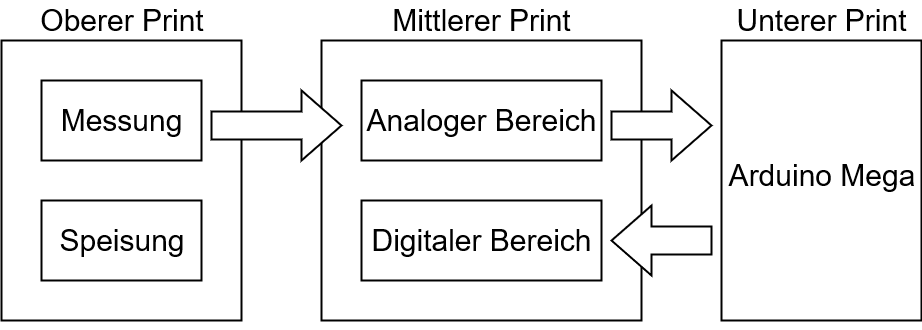
\includegraphics[width=0.9\textwidth]{images/Konzept_Elektrischer_Aufbau.png}
\caption{Konzept Elektrischer Aufbau}
\end{center}
\end{figure}


\subsection{Firmware Aufbau}
Domi neu Schreiben

[ Abbildung folgt noch ]  

\subsection{Software Aufbau}
Die Software stellt die Schnittstelle zwischen dem Menschen und dem P3T7 dar. Sie soll dazu dienen die Daten aus dem P3T7 zu lesen und sie für weitere Berechnungen bereitzustellen. Damit die Daten einfach weiterverarbeitbar sind, kann mithilfe der Software ein CSV-File generiert werden. Dieses kann leicht in Excel oder Matlab importiert werden. Des Weitern werden Berechnungen mit der Software gemacht, für welche der Controller zu schwach ist und um Speicherplatz auf dem P3T7 zu sparen.

\begin{figure}[H]
\begin{center}
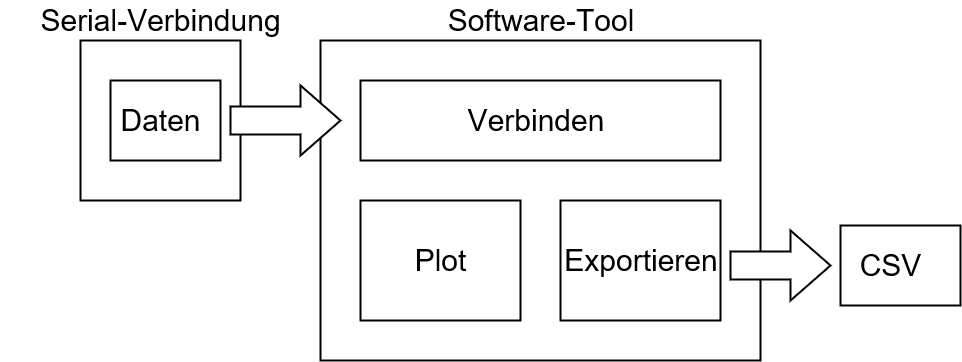
\includegraphics[width=0.9\textwidth]{images/Konzept_Software.png}
\caption{Konzept Software}
\end{center}
\end{figure}

Die Software stellt auch einen Plot mit den ausgelesenen Daten zur Verfügung. Der Plot soll dem User die Möglichkeit geben die Daten zu validieren, bevor er sie weiterverarbeitet. Die Software ist nicht geeignet, um die Daten zu verarbeiten.
\section{Technische Grundlagen}
%Elias Zusammenfassung kapitel
In den technischen Grundlagen kommen die verschiedenen Technologien und physikalischen Prinzipien zur Sprache, die verwendet wurden. 
\subsection{Hintergrund Messung}%Marc 1 Seite
Die Leistung kann auf verschiedene Arten, jedoch nicht direkt gemessen werden. Dieses Gerät misst die Leistung über den Momentanstrom und die Momentanspannung. Dabei wird folgende Formel verwendet.

\begin{equation}
	p(t) = u(t) \cdot i(t)
\end{equation}
\label{eq:Momentanleistung}

Damit kann die Leistung an einem bestimmten Zeitpunkt $t$ berechnet werden. Das Leistungsmessgerät soll jedoch die mittlere Leistung über zehn Sekunden berechnen. Um dies zu erreichen berechnet der Mikrocontroller die mittlere Leistung mittels folgender Grafik aufgezeigtem Algorithmus.
\begin{figure}[H]
\begin{center}
	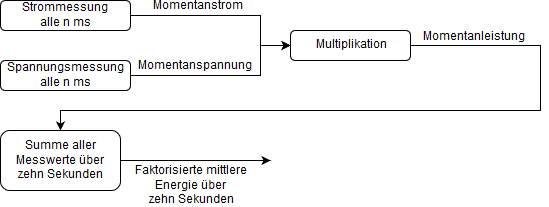
\includegraphics[width=100mm]{images/messung_schematisch.png}
	\caption{Algorithmus um mittlere Leistung zu berechnen} %picture caption
	\label{fig:berechnung_P}
\end{center}
\end{figure}

Wie in Abbildung \ref{fig:berechnung_P} ersichtlich, wird der Momentanstrom und die Momentanspannung alle \textbf{n (noch einfügen auch in Grafik)} Sekunden zusammenmultipliziert und die dabei erhaltene Momentanleistung über zehn Sekunden aufsummiert. Dieser Wert enspricht der faktorisierten geflossenen Energie über zehn Sekunden. Begründet ist dies durch folgende mathemetische Umformung.

\begin{equation}
	E = p(t) \cdot \Delta t
\end{equation}
\label{eq:energie1}

Mit der Annäherung, dass die Leistung $p(t)$ im Zeitraum zwischen zwei Messungen $\Delta t$ konstant ist und unter berücksichtigung der Formel \ref{eq:Momentanleistung}, ergibt sich folgende Berechnung der Energie.

\begin{equation}
	E_n = u_n \cdot i_n \cdot \Delta t
\end{equation}
\label{eq:energie2}

mit	$u_n, i_n = n $te Messung des Stromes und der Spannung.

Wenn nun alle $E_n$ aufaddiert werden ergibt sich die Energie über zehn Sekunden. Dabei kann $\Delta t$ ausmultipliziert werden.

\begin{equation}
	E_{10s}\quad = \sum_{n=1}^{ \frac{10s}{\Delta t} } E_n \quad = \quad \sum_{n=1}^{ \frac{10s}{\Delta t} } u_n \cdot i_n \cdot \Delta t \quad = \quad \Delta t \sum_{n=1}^{ \frac{10s}{\Delta t} } u_n \cdot i_n
\end{equation}
\label{eq:energie3}

\begin{equation*}
	\frac{E_{10s}}{\Delta t} = \sum_{n=1}^{ \frac{10s}{\Delta t} } u_n \cdot i_n \quad = \quad aE
\end{equation*}
	
Aus der vom Microkontroller berechneten Wert $aE$ lässt sich unter der verwendung der Formel $ \overline{P} = \frac{E}{t} $ die mittlere Leistung über zehn Sekunden $\overline{P}$ wie folgt berechnen.

\begin{equation}
	\overline{P}_{10s} = \frac{aE}{\Delta t \cdot 10s}
\end{equation}
\label{eq:mittlere_Leistung}
%%%%%%%%%%%%%%%%%%%%%%%%%%%%%%%%%%%%%%%%%%%%%%%%%%%%%%%%%%%%%%%%%%%%%%%%%%%

\subsection{Signalaufbereitung}%Elias 1 Seite
Die Signalaufbereitung passt die Messsignale an die Anforderungen des Analog-Digital-Wandlers, kurz ADC, an. Die Anforderungen sind gegeben, demnach wird die Schaltung an diese angepasst. So ist die zulässige Spannung am ADC 0V bis 5V. Diese Signalaufbereitungs-Strecke ist für die Strommessung und die Spannungsmessung identisch. Der einzige Unterschied zwischen den verschiedenen Signalen liegt in der Verstärkung.

\begin{figure}[H]
\begin{center}
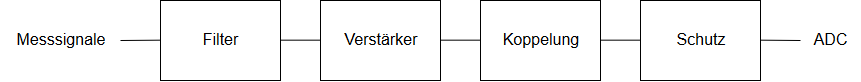
\includegraphics[width=0.9\textwidth]{images/Technische_Grundlagen_Signalaufbereitung.png}
\caption{Signalaufbereitungsstrecke}
\end{center}
\end{figure}

\subsubsection*{Filter}
Die Filter befreien das Messsignal von unerwünschten Signalanteilen. Da im Projektauftrag gefordert wird, dass harmonische Oberwellen ab 5kHz nicht gemessen werden, werden Filter diese Oberwellen entfernen. Dafür wurden Tiefpass-Filter 1. Ordnung verwendet.
\subsubsection*{Verstärkung}
Um die Messsignale auf eine brauchbare Grösse zu bringen, wurden Nicht-Invertierende Verstärker verwendet. Diese bringen den Vorteil, dass pro Messstrecke nur ein Operationsverstärker benötigt wird.
\subsubsection*{Koppelung}
Das erwartete Messsignal ist eine sinusartige Schwingung. Dadurch wird das Signal keinen DC-Anteil besitzen. Da der ADC Spannungen von 0 bis 5V fordert, muss das Messsignal angehoben werden.
\subsubsection*{Schutz}
Es ist eine Schutzschaltung eingebaut, um den ADC gegen Über- und Unterspannungen zu schützen. Diese entstehen in der Verstärkerschaltung bei den Messbereichen für kleine Ströme, wenn grosse Ströme gemessen werden.

\pagebreak
\section{Analoge Schaltung} 
\label{sec:analoge_schaltung}
Im Kapitel werden die verschiedenen analogen Schaltungsteile näher erläutert. Zuerst werden die verschiedenen Schaltungsteile auf dem Layer 1 erläutert. Dies beinhaltet die Speisung, Sicherheitsaspekte und die Messung. Danach werden die Bestandteile der Signalaufbereitung näher betrachtet.

\subsection{Layer 1}%Marc 1 Seite
%%%%%%%%%%%%%%%%%%%%%%%%%%%%%%%%%%%%%%%%%%%%%%%%%%%%%%%%%%%%%%%%%%%%%%%%%%%
Der erste Layer ist für alle Schaltungsteile mit 230V, sowie für die Verbindung nach aussen zuständig. Abbildung \ref{fig:first_layer} zeigt den groben Aufbau. Das genaue Schema befindet sich im Anhang.

\begin{figure}[H]
\begin{center}
	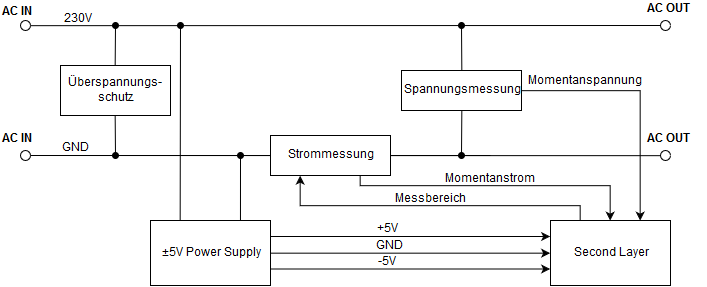
\includegraphics[width=160mm]{images/first_layer.png}
	\caption{Blockschaltbild des ersten Layers des Leistungsmessgerätes} %picture caption
	\label{fig:first_layer}
\end{center}
\end{figure}

\subsubsection*{Überspannungsschutz:}
Der Überspannungsschutz schützt das Gerät vor Spannungen über 400V. Der Rest des Gerätes ist somit für bis 400V ausgelegt. Da das Gerät mit Wechselstrom betrieben wird, ist ein Verpolungsschutz unnötig. Einzig wird die Masse des Gerätes auf 230VAC schweben, falls das Gerät verpolt betrieben wird.

\subsubsection*{Strommessung:}
Für die Strommessung stehen zwei Mess-Schunts zu Verfügung. Zum einen ein $50m\Omega$ Widerstand und zum anderen ein $1m\Omega$-Widerstand, welcher mit einem Relais parallel zum Ersten geschaltet wird. Durch die Parallelschaltung kann der Messbereich bei Betrieb umgeschaltet werden, ohne einen Unterbruch zu provozieren. Aufgrund induktiven Lasten könnten hohe Spannungen entstehen, die die Schaltung zerstören würden. Zudem kann somit eine unterbruchsfreie Versorgung der Last gewährleistet werden. Für die Messung wird die Spannung vor dem Shunt bezüglich Masse (GND) gemessen.

\subsubsection*{Spannungsmessung:}
Die Spannung wird durch einen Spannungsteiler mit dem Verhältnis $\frac{7.5}{1000}$ gemessen, was bei einer Spannung von $\pm 400V$ zu einem Messsignal von $\pm 3V$ führt. Da der Messbereich des ADCs $\pm 2.5V$ beträgt, können maximal Spannungen von $\pm 333V$ gemessen werden.

\subsubsection*{Power Supply:}
Das Netzteil versorgt den gesamten Gleichstromteil der Schaltung. Es stellt einen maximalen Strom von $400mA$ zur Verfügung.

%%%%%%%%%%%%%%%%%%%%%%%%%%%%%%%%%%%%%%%%%%%%%%%%%%%%%%%%%%%%%%%%%%%%%%%%%%%
\subsection{Filter}

Wie schon im Kapitel technische Grundlagen 3.2 erwähnt, werden die Filter benötigt um harmonische Oberwellen herauszufiltern. Gemäss Lastenheft sollen Oberwellen ab 5kHz nicht mehr im Signal sichtbar sein. Darum müssen Oberwellen die eine höhere Frequenz haben, unterdrückt werden damit diese nicht die Messung verfälschen.

\begin{figure}[H]
\begin{center}
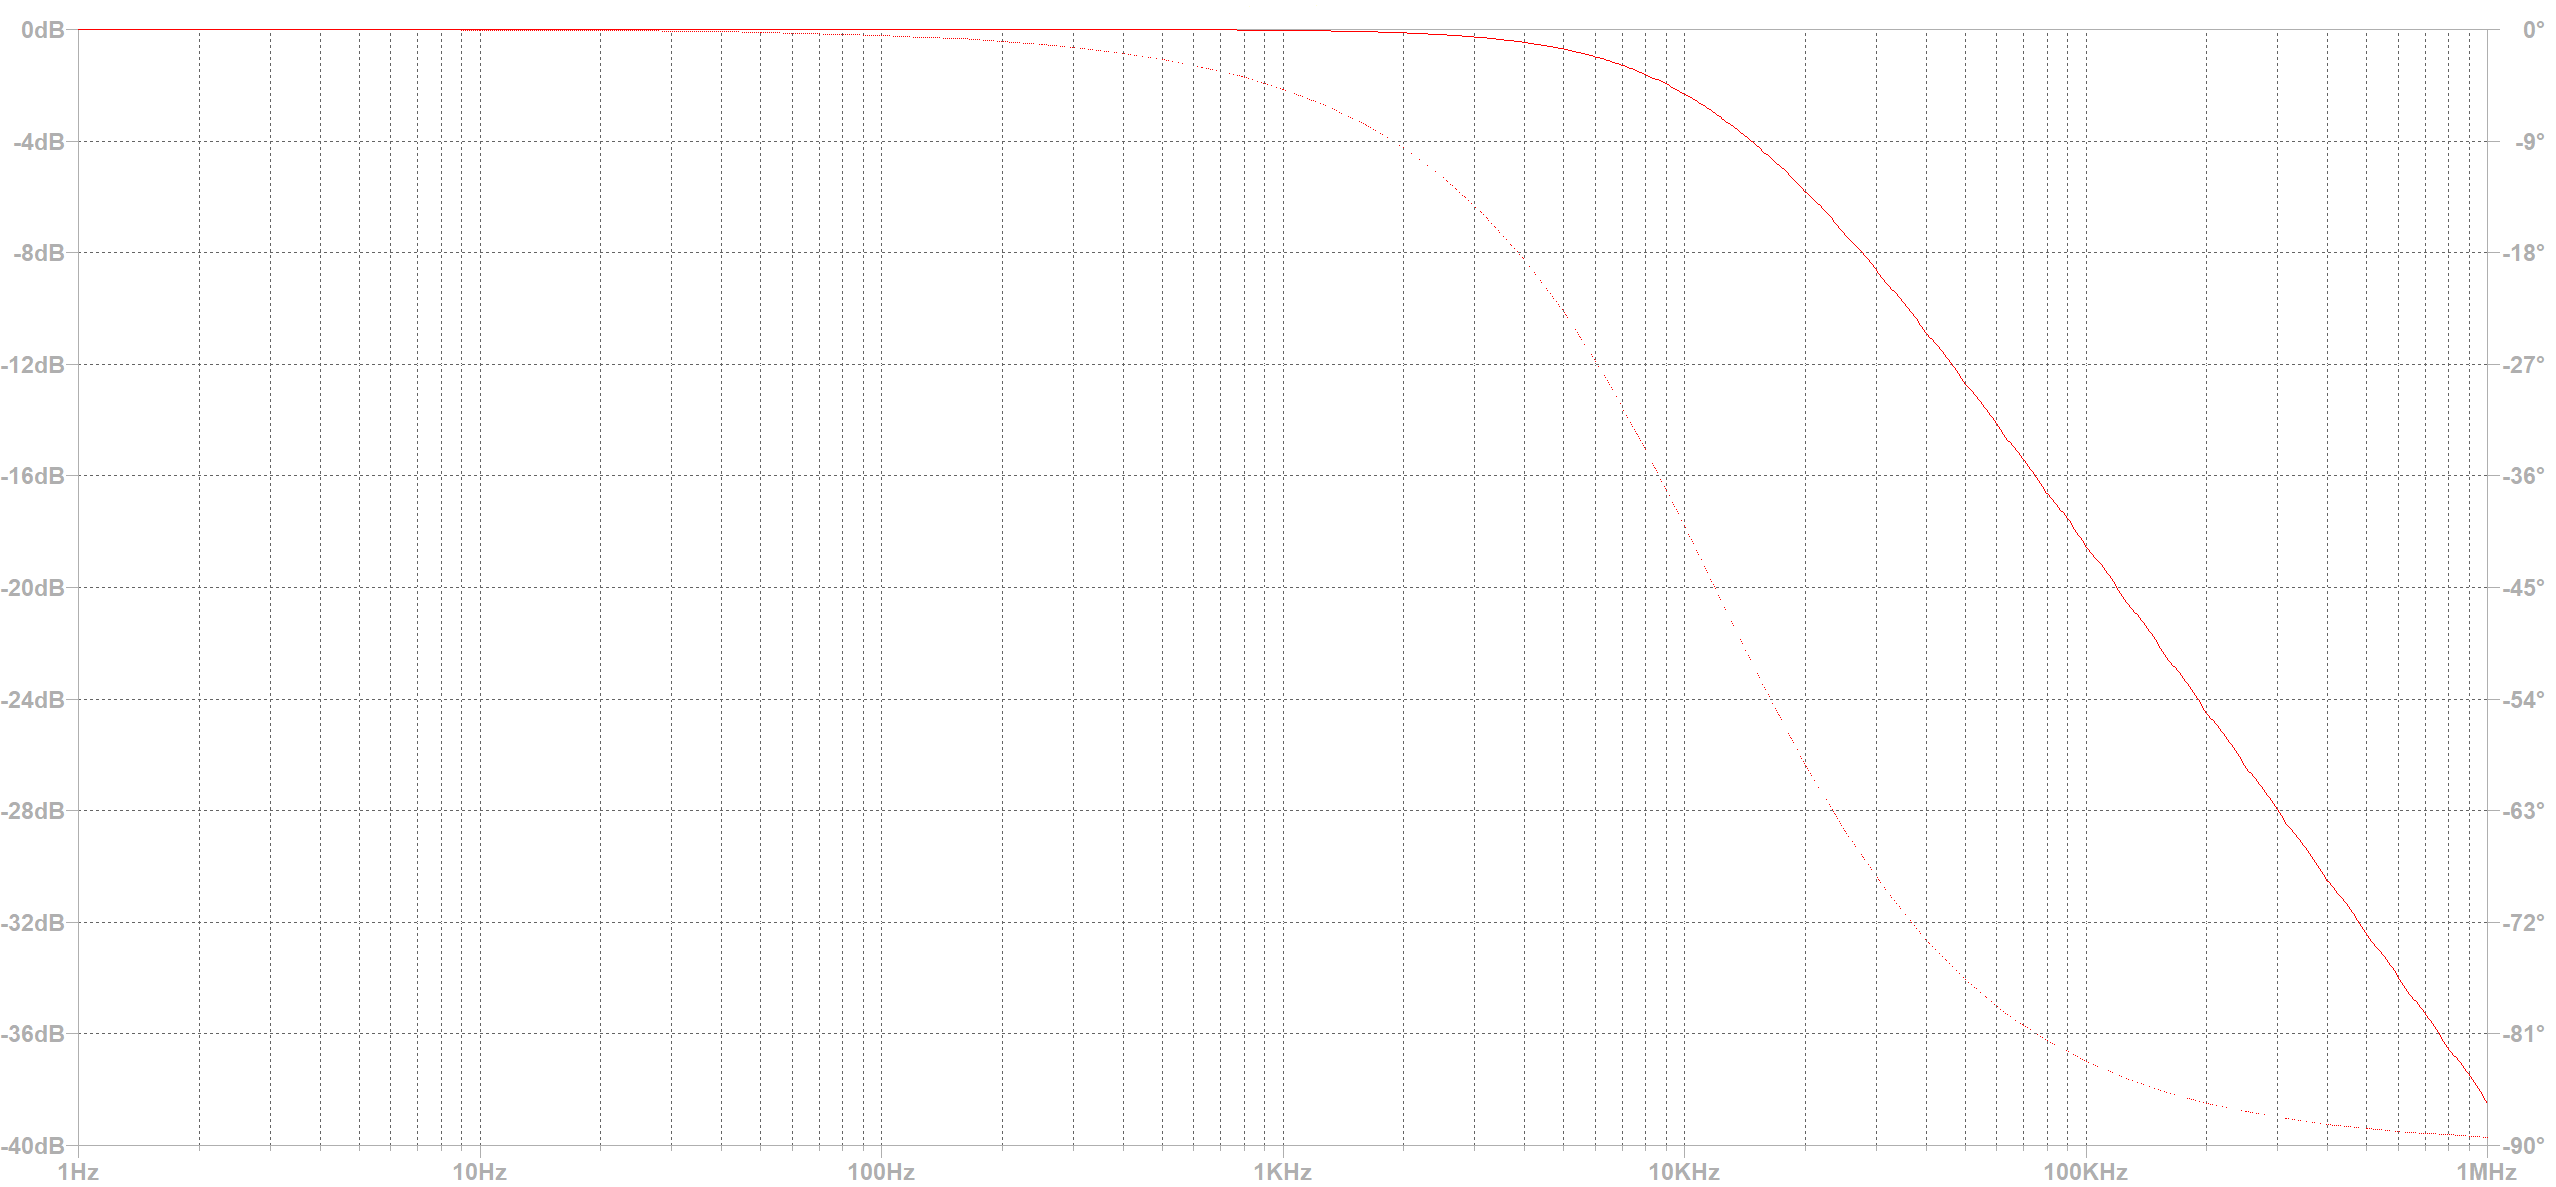
\includegraphics[width=0.9\textwidth]{images/Analoge_Schaltung_Frequenzgang.png}
\caption{Frequenzgang Tiefpass-Filter 1. Ordnung}
\end{center}
\end{figure}


Tiefpass-Filter sind geeignet, weil sie höhere Frequenzen unterdrücken und tiefe Frequenzen passieren lassen. Auf dem nebenstehenden Bild ist ein typischer Frequenzgang eines Tiefpass-Filters 1. Ordnung zu sehen. Da für das Projekt die Signale auch verstärkt werden müssen, sind aktive Filter naheliegend.\cite{ant}


\subsubsection*{Dimensionierung}

Die Wahl fiel auf Butterworth-Filter mit Sallen/Key-Topologie 2. Ordnung. Diese Topologie bietet den Vorteil, dass sie nicht invertierend ist. Dadurch ist ein Operationsverstärker ausreichend pro Signalpfad. Die Butterworth-Koeffizienten bieten den Vorteil, dass sie flach sind im Durchlassbereich und einen relativ eckigen Übergang haben.\cite{wiki}



\begin{figure}[H]
\begin{center}
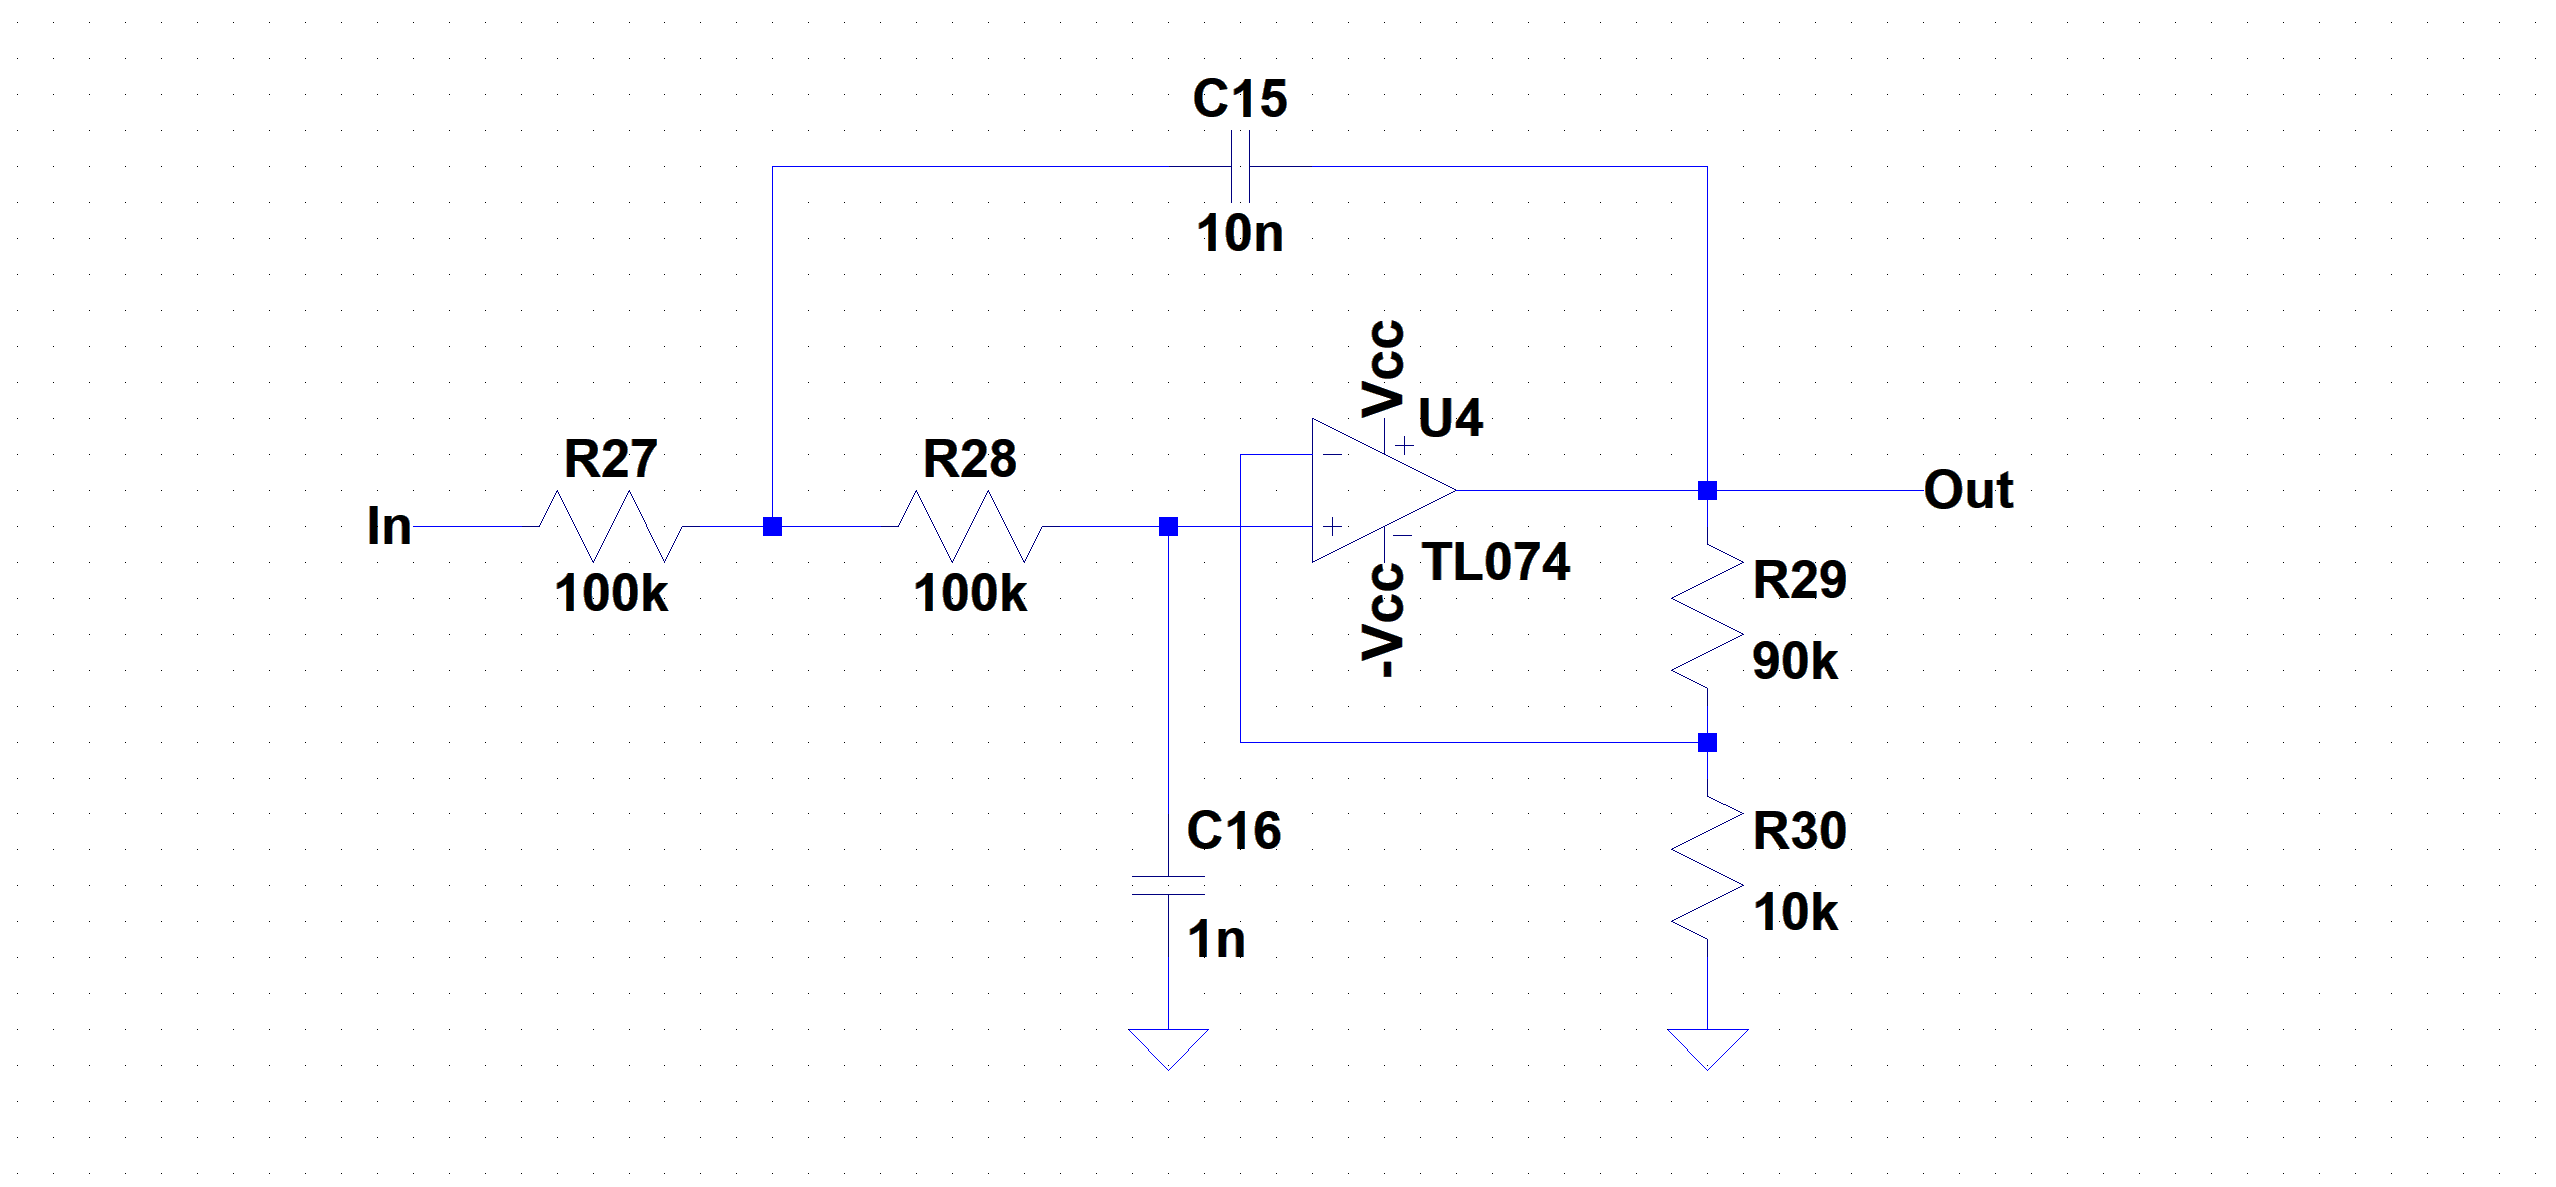
\includegraphics[width=0.9\textwidth]{images/Analoge_Schaltung_Sallen.png}
\caption{Sallen/Key-Topologie Tiefpass-Filter 2. Ordnung}
\end{center}
\end{figure}


\subsubsection*{Auswahl Operationsverstärker}
An den Operationsverstärker wurden praktisch keine Anforderungen gestellt. Er soll ein GWP\cite{wiki} von mindestens 800kHz besitzen und nicht Rail-to-Rail sein. Ausserdem werden vier Operationsverstärker benötigt. Dies ist der \textbf{TL074}, der praktischerweise 4 Operationsverstärker in einem Gehäuse vereint. Die passiven Bauteile wurden mithilfe einer Formel\cite{fail} aus dem Internet erstellt, die sich im Laufe des Projektes als falsch herausstellte.

\subsubsection*{Falsche Filter}
Nachdem der Print gefertigt war, wurde beim Testen festgestellt, dass die Filter instabil laufen. Es wurde überlesen, dass mit der Sallen/Key-Filtertopologie nur Verstärkungen bis drei realisierbar sind. Bei höheren Verstärkungen können diese instabil werden. Diesen schwerwiegenden Fehler wurde gemacht. Aus der Not wurden die Filter umgebaut in einen passiven Filter 1. Ordnung, gefolgt von einer Verstärkerschaltung. Dafür musste nur der Kondensator C15 entlötet werden, damit ein Unterbruch entsteht, und für den R27 wurde eine Drahtbrücke eingelötet.

\begin{figure}[H]
\begin{center}
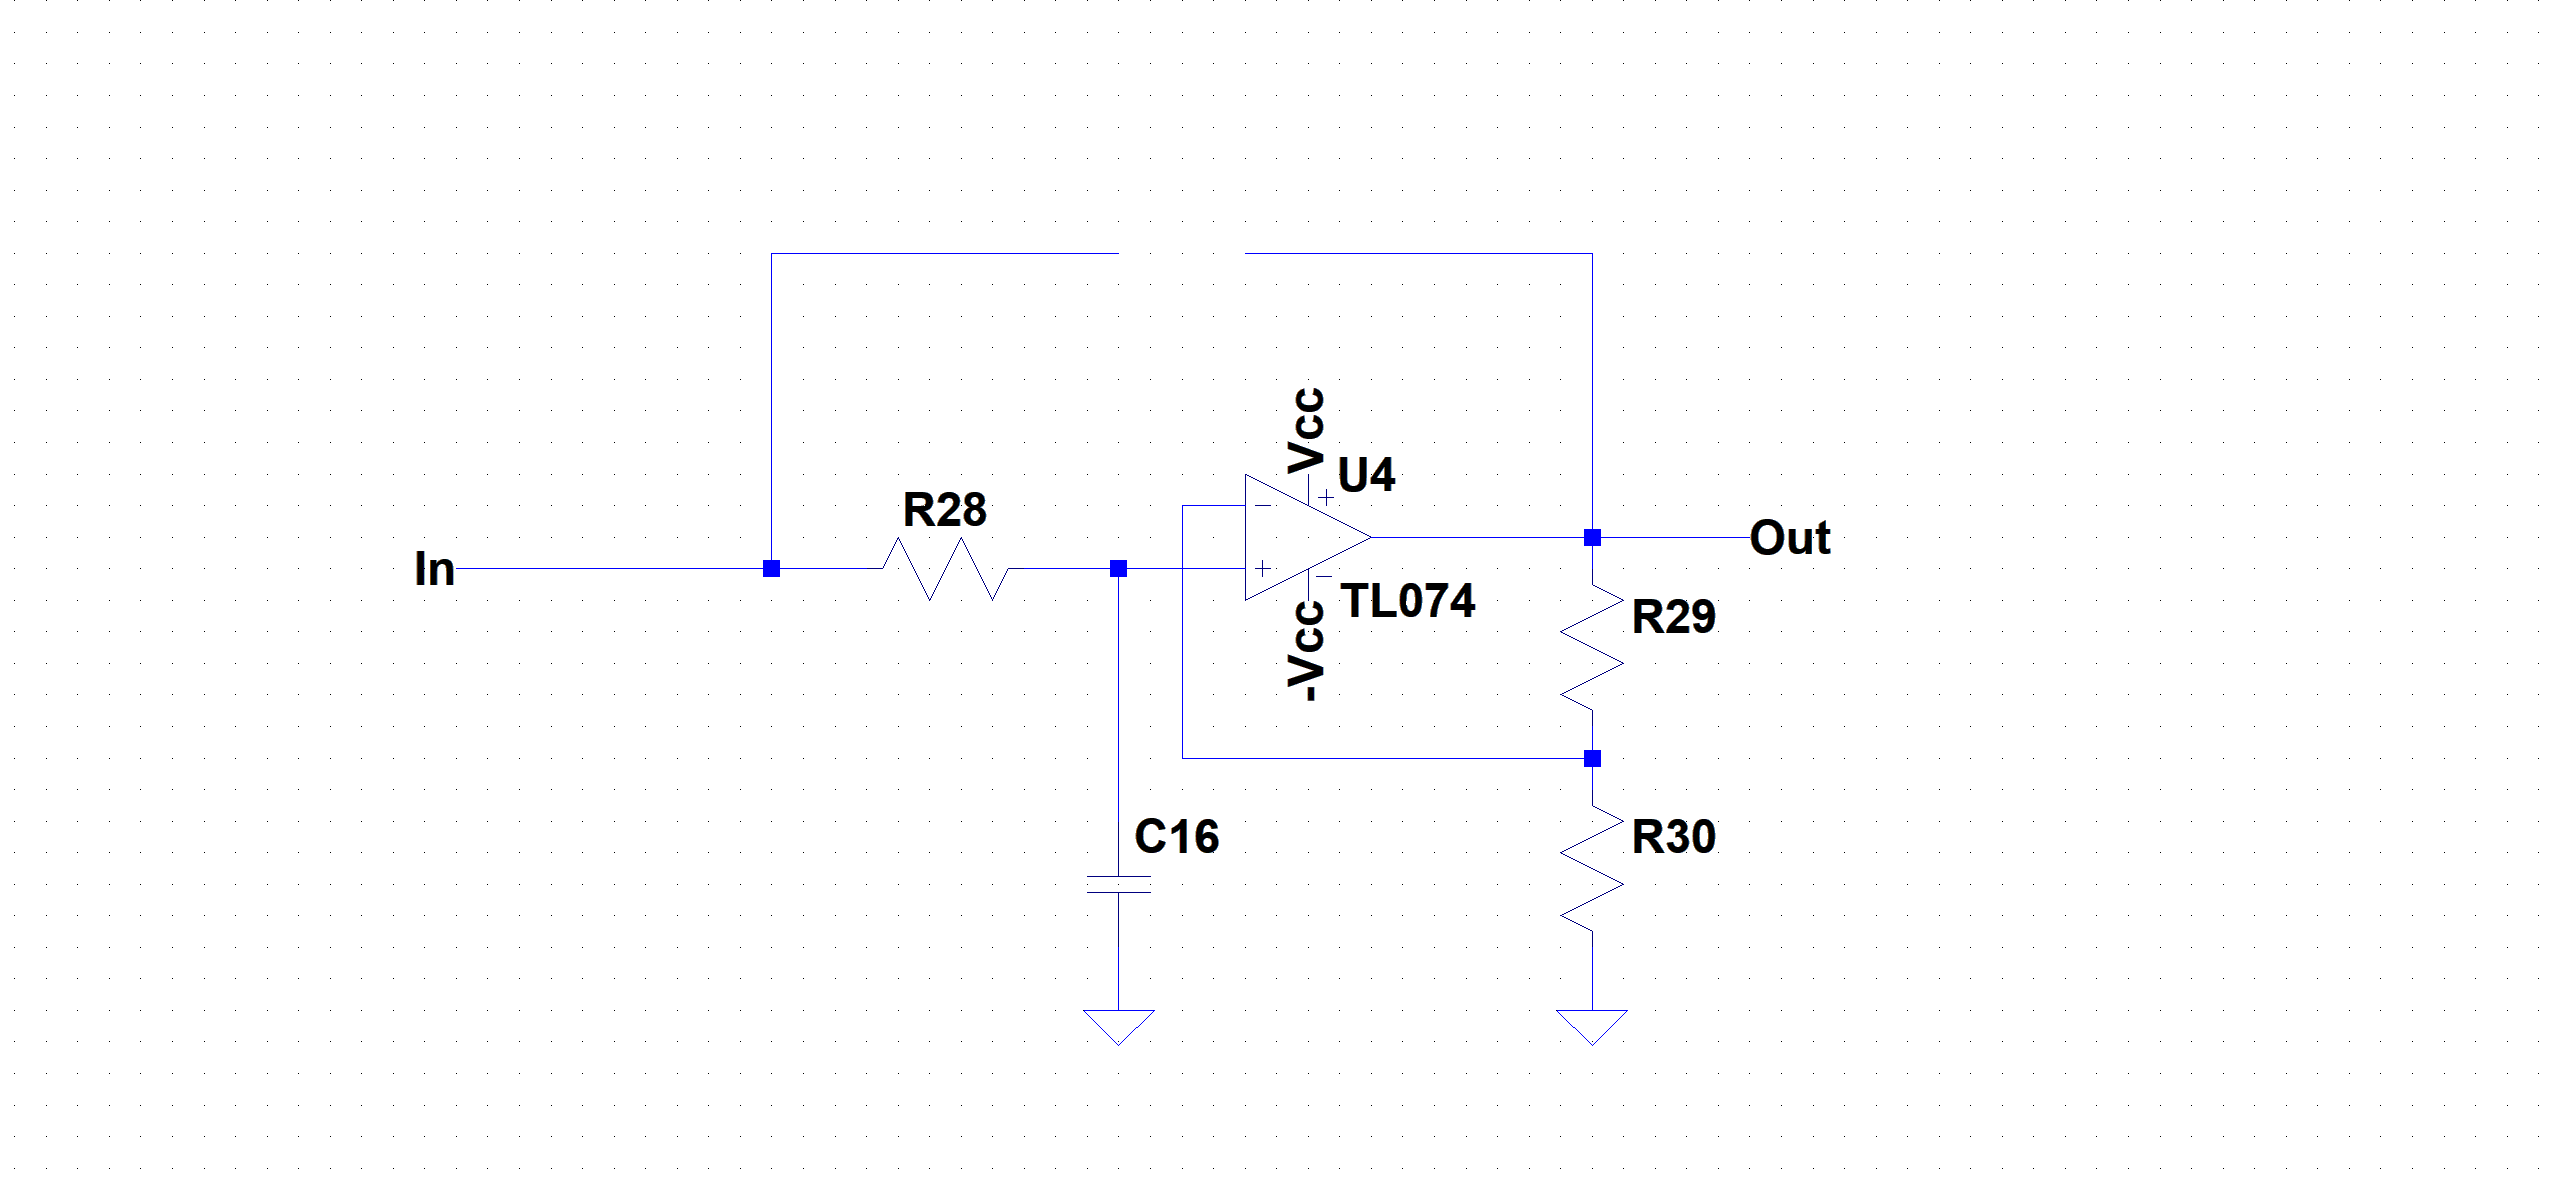
\includegraphics[width=0.9\textwidth]{images/Analoge_Schaltung_Sallentopassive.png}
\caption{Umgebautes Sallen/Key zu passivem Filter 1. Ordnung}
\end{center}
\end{figure}

Die Dimensionierung der neuen Schaltung ist mithilfe der nachfolgenden Formeln geschehen. Die Verstärkungen konnten beibehalten werden. Die passiven Filter mussten neu berechnet werden.\cite{wiki}

\begin{equation}
f_g=\frac{1}{2 \cdot \pi \cdot R_{28} \cdot C_{16}}
\label{eq:Grenzfrequenz}
\end{equation}

\begin{equation}
A=1+\frac{R_{29}}{R_{30}}
\label{eq:Verstärkung}
\end{equation}

%%%%%%%%%%%%%%%%%%%%%%%%%%%%%%%%%%%%%%%%%%%%%%%%%%%%%%%%%%%%%%%%%%%%%%%%%%%
\subsection{Einkoppelung}
Das Signal nach der Filterung und der Verstärkung beträgt $\pm 2.5V$. Um dieses Signal anzuheben auf eine für den Mikrocontroller angepasste Grösse, wird eine DC-Spannung eingekoppelt. Nach der Einkoppelung von $2.5V$ bewegt sich das Signal innerhalb von $0V$ bis $5V$. Dies wurde mit folgender Schaltung realisiert, siehe Abbildung \ref{fig:Einkoppelung}.


\begin{figure}[H]
\begin{center}
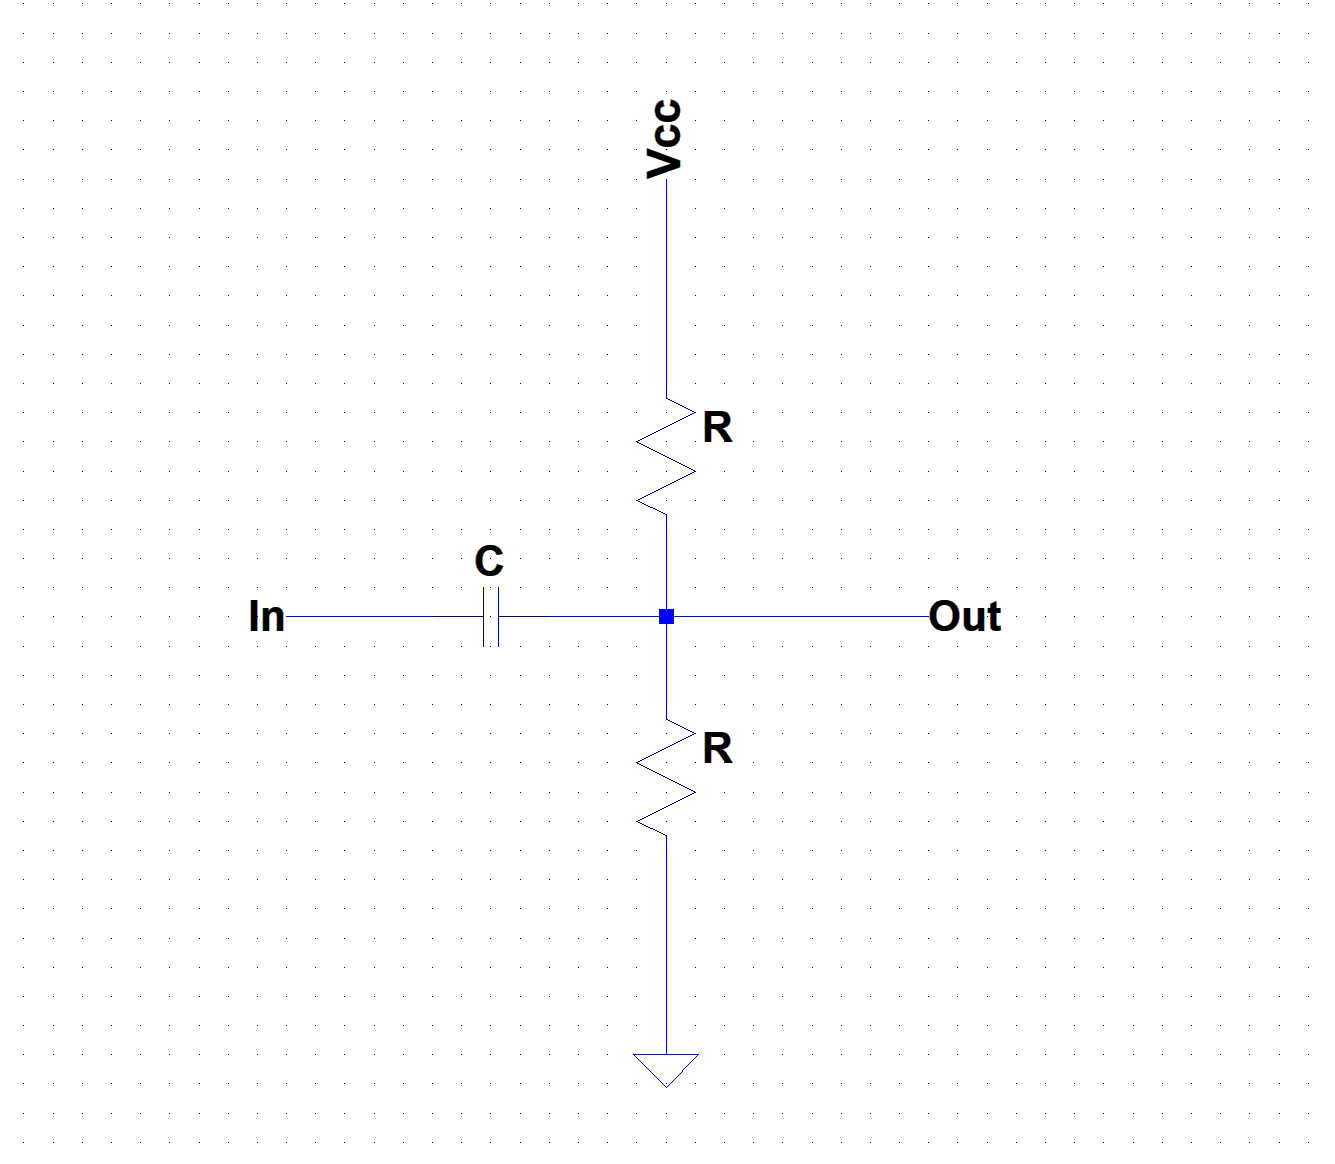
\includegraphics[width=0.9\textwidth]{images/Analoge_Schaltung_Einkoppelung.png}
\caption{Einkoppelung}
\label{fig:Einkoppelung}
\end{center}
\end{figure}

Um diese Schaltung zu dimensionieren, muss eine AC- und eine DC-Betrachtung gemacht werden.


Für die AC-Betrachtung ist sie ein Hochpassfilter 1. Ordnung. Dieses Hochpassfilter soll alle Frequenzen passieren lassen ausser Gleichstrom. Für die Dimensionierung kann dieselbe Formel \eqref{eq:Grenzfrequenz} wie für die Tiefpass-Filter verwendet werden. Jedoch wird die Grenzfrequenz $f_g$ auf $0.5 Hz$ gesetzt. $R_{28}$ setzt sich aus den  zwei parallel gesetzten Widerständen zusammen.


Für die DC-Betrachtung entspricht die Schaltung einem Spannungsteiler. Der Kondensator stellt in dieser Betrachtung einen Unterbruch dar. Die Widerstände sollten gross gewählt werden, damit die Verluste klein bleiben. Gleichzeitig muss mit den Anforderungen des Hochpassfilters einen Kompromiss gefunden werden. Für unser Projekt war schlussendlich die Grösse des Kondensators ausschlaggebend. Je grösser der Kondensator ist desto kleiner wird die Verlustleistung. Der grösste Kondensator der als SMD\cite{wikiSMD} erhältlich ist wurde verwendet.

%%%%%%%%%%%%%%%%%%%%%%%%%%%%%%%%%%%%%%%%%%%%%%%%%%%%%%%%%%%%%%%%%%%%%%%%%%%
\subsection{Sicherheitsschaltung}

Um die Eingänge des Mikrocontroller zu schützen, wurde eine Sicherheitsschaltung realisiert. Diese schützt den Eingang vor Überspannungen und Unterspannungen. Die obere Diode schaltet, sobald das Eingangssignal oberhalb von Vcc plus der Forward-Voltage der Diode ist. In diesem Fall entsteht ein Kurzschluss zwischen GND und Vcc durch den Operationsverstärker. Um den Strom zu begrenzen, ist der Widerstand vorhanden. Gleichzeitig bildet der Widerstand mit dem Kondensator zusammen ein weiteres Tiefpass-Filter, das hochfrequente Störungen abhalten soll.  Die Grenzfrequenz dieses Filters muss höher sein, als die Grenzfrequenz des ersten Filters, damit es nicht das Signal verfälscht.


\begin{figure}[H]
\begin{center}
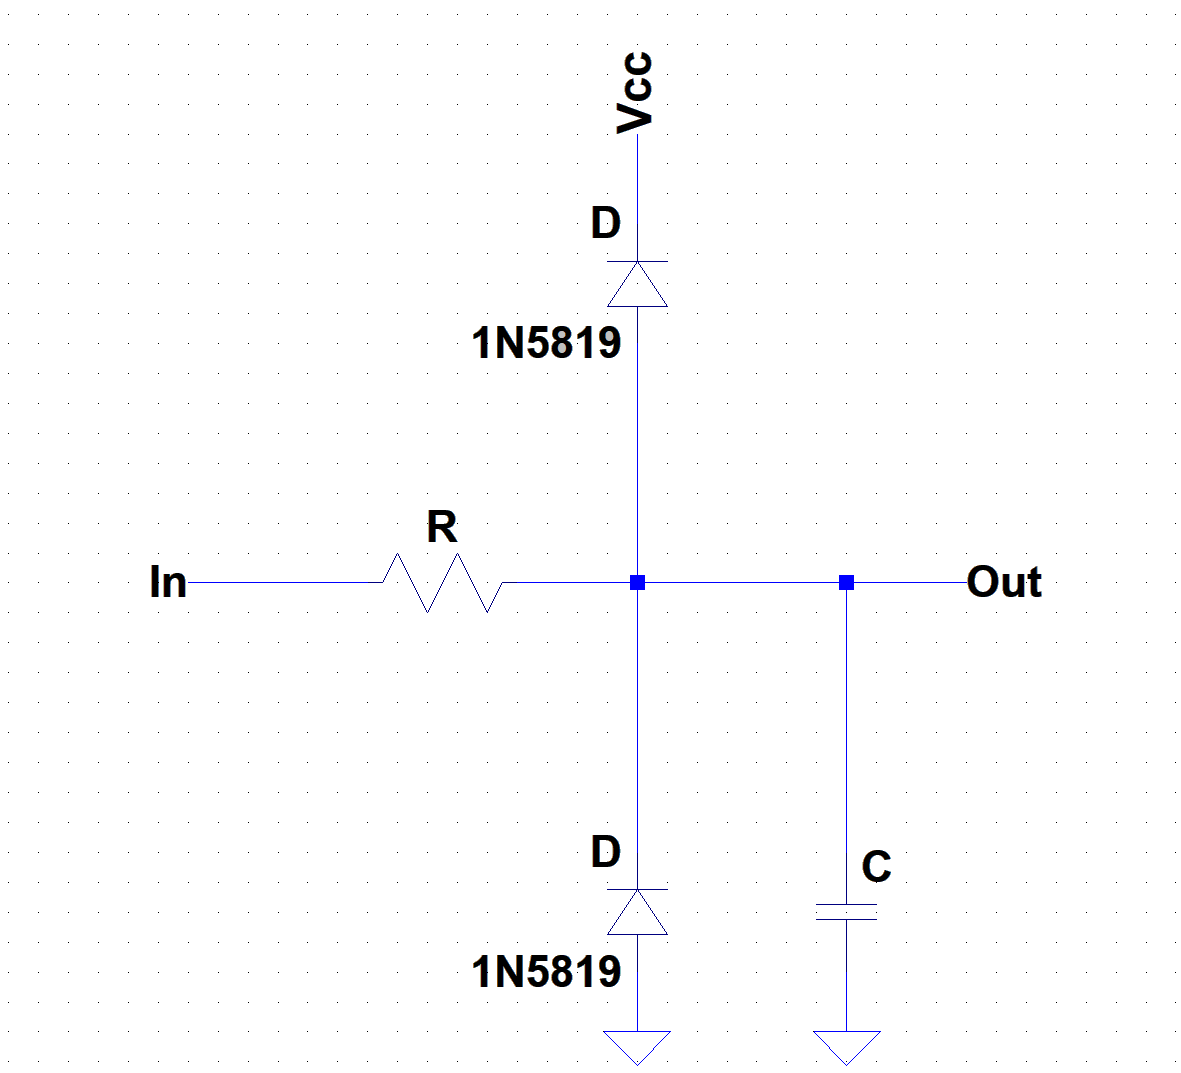
\includegraphics[width=0.9\textwidth]{images/Analoge_Schaltung_Sicherung.png}
\caption{Sicherheitsschaltung}
\label{fig:Sicherheitsschaltung}
\end{center}
\end{figure}

\subsection{Genauigkeit}%Marc 1 Seite
%%%%%%%%%%%%%%%%%%%%%%%%%%%%%%%%%%%%%%%%%%%%%%%%%%%%%%%%%%%%%%%%%%%%%%%%%%%
Die Genauigkeit im analogen Schaltungsteil hängt zum einen von den Toleranzen und Ungenauigkeiten der verwendeten Bauteile und zum anderen von der Auflösung des ADCs ab, welcher die Grenze zwischen analog und digital bildet. Abbildung \ref{fig:genauigkeit} zeigt den Messpfad mit den möglichen Teilen, in welchen Ungenauigkeiten entstehen können und werden.

\begin{figure}[htb]
	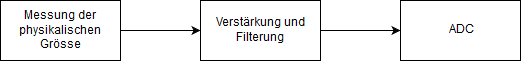
\includegraphics[width=160mm]{images/Analoge_Schaltung_genauigkeit.png}
	\caption{Messpfad} %picture caption  
	\label{fig:genauigkeit}
\end{figure}

Nachfolgend werden die möglichen Fehler der einzelnen Blöcke in Abbildung \ref{fig:genauigkeit} erläutert.

\subsubsection*{Messung der physikalischen Grösse}
Der Strom und die Spannung werden jeweils als Spannung über einen bestimmten Widerstand gemessen.Wie aus dem Schema im Anhang ersichtlich, lässt sich der Strom über das Ohmsche Gesetz berechnen und die Spannung über einen Spannungsteiler. 

\begin{equation}
I = \frac{U_{mess}}{R_{mess}} \to I = \frac{U_{mess}}{R_{mess} + R_{toleranz}} = \frac{U_{mess}}{R_{mess}} \cdot \frac{1}{a}
\end{equation}

\[a = \frac{R_{mess} + R_{toleranz}}{R_{mess}}\]

\begin{equation}
U = U_{mess} \cdot \frac{R_{tot}}{R_{mess}} \to U = U_{mess} \cdot \frac{R_{tot} + R_{toleranz1,2}}{R_{mess}+R_{toleranz2}} = U_{mess} \cdot \frac{R_{tot}}{R_{mess}} \cdot \frac{1}{b}
\end{equation}

\[b = \frac{\frac{R_{tot} + R_{toleranz1,2}}{R_{tot}}}{\frac{R_{tot} + R_{toleranz2}}{R_{tot}}}\]

Somit ergeben die Toleranzen der Widerstände konstante faktorielle Fehler $a$ und $b$, welche durch eine Multiplikation während der digitalen Weiterverarbeitung des Messsignals behoben werden können.





\subsubsection*{Verstärkung, Einkopplung und Filterung}
Der Strom und die Spannung werden im jeweiligen Kanal verstärkt, um 2.5V angehoben und gefiltert. Da die Filterung erst ab 10kHz abschneidet, sind die Fehler im Durchlassbereich vernachlässigbar. Die Verstärkung wird durch einen nicht invertierenden Operationsverstärker erreicht.

\begin{equation}
U_{out} = U_{in} \left( 1+\frac{R_2}{R_1} \right) \to U_{out} = U_{in} \left( 1+\frac{R_2+R_{toleranz1}}{R_1+R_{toleranz2}} \right) = U_{in}\left(1+\frac{R_2}{R_1}\right) \cdot \frac{1}{a}
\end{equation}

Somit kann der Fehler wie im vorherigen Abschnitt durch eine Multiplikation mit einer Konstante kompensiert werden.

Bei der Einkopplung wird die Spannung an einem Spannungsteiler zum Signal hinzuaddiert (siehe Schema im Anhang).

\begin{equation}
U_{out} = U_{in} + \frac{V_{CC} \cdot R_2}{R_1+R_2} \to U_{out} = U_{in} + \frac{V_{CC} \cdot (R_2 + R_{toleranz2})}{R_1+R_2 + R_{toleranz1,2}} =  U_{in} + \frac{V_{CC} \cdot R_2}{R_1+R_2} + b
\end{equation}

Daher wird bei diesem Fehler im Gegensatz zu den anderen eine zusätzliche Konstante dazu addiert, um den durch die Widerstandstoleranzen entstandenen Fehler zu entfernen.
 
\subsubsection*{Analog-Digital-Wandler}
Bei der Konvertierung eines analogen Signals zu einem Digitalem gibt es zwingendermassen einen Informationsverlust durch die Quantisierung des Signals. Da für dieses Gerät ein 10 Bit ADC verwendet wird, hat das digitale Signal eine Auflösung von 1024 Werten. Für die vier Messkanäle ergeben sich folgende Toleranzen in der Tabelle \ref{tab:auflösung}.


\begin{table}[H]
\centering
\begin{tabular}{|l|l|l|l|l|}
\hline
Messung     & Spannung  & \multicolumn{3}{c|}{Strom}     \\ \hline
Messbereich & $\pm333V$ & $\pm15A$ & $\pm5A$ & $\pm0.5A$ \\ \hline
Auflösung   & $0.65V$   & $29mA$   & $9.8mA$ & $0.98mA$  \\ \hline
\end{tabular}
\caption{Auflösung der Messbereiche}
\label{tab:auflösung}
\end{table}

\subsubsection*{Resultierende Genauigkeit} 
Die Ungenauigkeit setzt sich zum einen durch den Informationsverlust der Quantisierung am ADC zusammen. Zum Anderen werden zusätzliche Ungenauigkeiten durch elektromagnetische Einkopplungen der umgebenden Schaltung und nicht einberechnete Faktoren der Schaltung wie zum Beispiel Leitungswiderstände entstehen. Die Fehler, welche durch die Toleranzen der Bauteile entstehen, können wie in den vorherigen Abschnitten beschrieben durch Multiplikationen und Additionen kompensiert werden.



\pagebreak
\section{Software}
Die Firmware des Messgerätes ist eine in C geschriebene Software für die AVR-Prozessor-architektur. Sie besteht aus einem Hauptprogramm zur Ablaufsteuerung und mehreren C-Modulen für die Kommunikation mit den Peripheriegeräten sowie diverse Algorithmen. Die Bediensoftware ist eine Java-Applikation für Windows.

\subsection{Berechnungskonzept}
Einer der Hauptaugenmerke der Firmware ist die Effizienz. Je schneller der Code arbeitet, desto höher kann die Abtastfrequenz sein und desto genauer wird die Messung. Eigens für das Messgerät wurde deshalb ein schlankes Übertragunsprotokoll sowie eine Berechnungsgrundlage entwickelt, dessen Ziel eine möglichst effiziente Verarbeitung der Messdaten ist. Nachfolgend erfolgt die Herleitung und Funktionsweise dieses Konzepts.
Der verwendete Mikrocontroller besitzt eine einfache 8Bit CPU ohne Floating Point Unit. Das heisst, er besitzt keine Recheneinheit, die Operationen auf Gleitkommazahlen direkt anwenden kann. Deshalb sorgt erste Optimierung dafür, dass die Firmware möglichst nur mit Ganzzahlen arbeitet und eine Umrechnung in die Leistung mit Nachkommastellen erst ganz am Schluss erfolgt.

Zunächst muss eine Grenze gezogen werden bezüglich der Genauigkeit der Messdaten. Die erste Einschränkung erfolgt durch die Quantisierung des ADC. Dieser hat beim ATMega2560 eine Auflösung von 10Bit. Digitalisiert werden drei Strombereiche und die Spannung. Je nach Bereich ergibt sich dadurch eine (theoretische) Genauigkeit pro Bit. Die Daten können aus Tabelle \ref{tab:theoretische_Genauigkeit_der_Messbereiche} entnommen werden.


\begin{table}[H]
\begin{center}
\begin{tabular}{|l|l|l|l|l}
\cline{1-4}
Analoger Eingang & Beschreibung           & Wertebereich   & $r_{ADC}$ Auflösung pro Bit &  \\ \cline{1-4}
ADC0             & Spannung               & -400V bis 400V & 0.78125$\frac{V}{Bit}$      &  \\ \cline{1-4}
ADC1             & Kleinster Strombereich & -0.5A bis 0.5A & 0.0009765625$\frac{A}{Bit}$ &  \\ \cline{1-4}
ADC2             & Mittlerer Strombereich & -5A bis 5A     & 0.009765625$\frac{A}{Bit}$  &  \\ \cline{1-4}
ADC3             & Grösster Strombereich  & -15A bis 15A   & 0.029296875$\frac{A}{Bit}$  &  \\ \cline{1-4}
\end{tabular}
\caption{theoretische Genauigkeit der Messbereiche}
\label{tab:theoretische_Genauigkeit_der_Messbereiche}
\end{center}
\end{table}


Das Messgerät speichert keine Strom- oder Spannungswerte ab, sondern nur die Leistung. Die Werte von Abbildung \ref{tab:theoretische_Genauigkeit_der_Messbereiche} können deshalb noch für jeden Bereich multipliziert werden. Man erhält dadurch die Genauigkeit der Leistung pro Bit.

\begin{equation}
R_{ADC1}=r_{ADC0}\cdot r_{ADC1}= 0.000762939\frac{W}{Bit}
\label{eq:RADC1}
\end{equation}
\begin{equation}
R_{ADC2}=r_{ADC0}\cdot r_{ADC2}= 0.007629394\frac{W}{Bit}
\label{eq:RADC2}
\end{equation}
\begin{equation}
R_{ADC3}=r_{ADC0}\cdot r_{ADC3}= 0.022888184\frac{W}{Bit}
\label{eq:RADC3}
\end{equation}

Die Analogschaltung bildet die verschiedenen Wertebereiche in ein Intervall von $0V$ bis $5V$ ab. Der AD-Wandler ist so eingestellt, dass dieser die Eingangsspannung bezogen auf eine Referenzspannung von $5V$ digitalisiert. Der zugewiesene Dezimalwert ist durch Formel \ref{eq:ADC} gegeben. Die Eingangsspannung variiert je nach Wertebereich und kann durch Formel \ref{eq:UIN} reproduziert werden. Zur übersichtlicheren und allgemeinen Darstellung wurde dem realen Signal die Variable x zugeordnet.

\begin{equation}
ADC=\frac{U_{IN} \cdot 2^{10}}{U_{ref}}
\label{eq:ADC}
\end{equation}

\begin{equation}
U_{IN} =\frac{U_{ref}}{x_{max} - x_{min}} \cdot \left( x + \frac{x_{max} - x_{min}}{2} \right) = \frac{U_{ref} \cdot x}{x_{max} - x_{min}}+\frac{U_ref}{2}
\label{eq:UIN}
\end{equation}

\begin{table}[H]
\begin{tabular}{ll}
ADC:		&  Registerwert dezimal [ ]\\
$U_{IN}$:	&  Eingansspannung am ADC [V]\\
x:			&  Realer Signalwert [V]oder [A]\\
$U_{ref}$:	&  Referenzspannung entspricht 5V\\
\end{tabular}
\end{table}

Die Schreibweise $x_{max}-x_{min}$ bezeichnet den Wertebereich des entsprechenden Eingangs, wie er in Abbildung \ref{tab:theoretische_Genauigkeit_der_Messbereiche} gezeigt ist. Da die Analogschaltung ein offsetbelastetes Eingangssignal liefert (2.5V am ADC entsprechen 0A bzw. 0V), muss dieser entfernt werden. Die beiden Gleichungen \ref{eq:ADC} und \ref{eq:UIN} werden kombiniert und algebraisch umgeformt.

$$ ADC=\frac{U_{IN} \cdot 2^{10}}{U_{ref}}=\frac{U_{ref} \cdot x}{x_{max} - x_{min}}+\frac{U_ref}{2} \cdot \frac{ 2^{10}}{U_{ref}}=\frac{x \cdot 2^{10}}{x_{max} - x_{min}}+\frac{2^{10}}{2}$$

$$ADC-\frac{2^{10}}{2}=ADC-512=x \cdot \frac{2^{10}}{x_{max} - x_{min}}$$

Es genügt somit, nur den Dezimalwert des ADCs abzüglich des Offsets in den Buffern zu speichern. Der gesamte rechte Teil ist vorerst redundant und kann am Ende wieder hinzugefügt werden. Dies bedingt jedoch auch, dass man für jeden Wertebereich einen eigenen Buffer benötigt, da jeder Buffer eine andere Wertigkeit pro Bit aufweist. Möchte man aus dem Dezimalwert des ADC den realen Wert zurückbilden, so muss die Gleichung nur auf x umgeformt werden.

$$x=(ADC-512)\cdot \frac{x_{max} - x_{min}}{2^{10}}=(ADC-512)\cdot r_{ADCn}$$

Dieser Skalierungsfaktor entspricht genau der in Abbildung \ref{tab:theoretische_Genauigkeit_der_Messbereiche} gezeigten Genauigkeit pro Bit. Da nach der Offsetentfernung das System nun linear ist, können die Dezimalwerte der einzelnen Eingänge ebenfalls multipliziert werden. Somit gilt:

\begin{equation}
p_i=(ADC0-512)\cdot(ADCn -512) \cdot r_{ADC0} \cdot r_{ADCn} = (ADC0-512)\cdot(ADCn -512) \cdot R_{ADCn}
\label{eq:PI}
\end{equation}

Wie bereits erwähnt basiert das Berechnungskonzept auf das Aufsummieren der Momentanleistung über eine bestimmte Zeit. Physikalisch betrachtet wird also zwischenzeitlich die Energie gespeichert und nicht die Leistung. Ist wie in unserem Fall die Messung zeitdiskret, so gilt:

\begin{equation}
E=\sum_{i=1}^{f_s \cdot t_s} p_i \cdot\Delta t = \sum_{i=1}^{f_s \cdot t_s} (ADC0-512)\cdot(ADC1 -512) \cdot R_{ADCn} \cdot \frac{1}{f_s}
\label{eq:E}
\end{equation}

\begin{table}[H]
\begin{tabular}{ll}
E:			&  Energie [J]\\
$p_i$:		&  Eingansspannung am ADC [V]\\
$\Delta t$:	&  Zeitdifferenz [s]\\
$f_s$:		&  Abtastfrequenz [Hz]\\
$ R_{ADCn} $: & Wertigkeit des Buffers [$\frac{W}{Bit}$]\\
$t_s$:		&  Abtastzeit [s]
\end{tabular}
\end{table}

Formel \ref{eq:E} wird nun auf beiden Seiten erweitert und wieder algebraisch umgeformt.

$$E=\sum_{i=1}^{f_s \cdot t_s} p_i \cdot \frac{1}{f_s}$$

$$\frac{f_s}{R_{ADCn}}\cdot E =\frac{f_s}{R_{ADCn}}\cdot \sum_{i=1}^{f_s \cdot t_s} p_i \cdot \frac{1}{f_s} = \sum_{i=1}^{f_s \cdot t_s} \frac{p_i}{R_{ADCn}} = \sum_{i=1}^{f_s \cdot t_s} (ADC0-512)\cdot(ADC1 -512)$$

Innerhalb des Summenoperators befindet sich nun genau der in Formel \ref{eq:PI} hergeleitete Wert des Buffers. Da Leistung bekanntlich Energie durch Zeit ist, muss man den Term nur noch auf diesen Ausdruck umformen und man erhält die reale Leistung des Eingangssignals. Dem gesamten rechten Ausdruck der Gleichung wurde die Variable B zugewiesen. B ist der Dezimalwert im Buffer, nachdem dieser 10 Sekunden lang aufsummiert wurde.

\begin{equation}
\overline{P} = \frac{E}{t_s} = B \cdot \frac{R_{ADCn}}{f_s \cdot t_s}
\label{eq:P}
\end{equation}

Das Problem dieses Konzeptes ist der grosse Dynamikbereich. Wenn man die Messwerte aufsummiert, können im "worst case"  bis zu 35Bit grosse Zahlen im Buffer entstehen (bei 10kHz Abtastfrequenz und 10s Abtastzeit). Als Alternative könnte man die einzelnen Buffer abspeichern und die Rückskalierung erst in der Java-Applikation vornehmen. Um Speicherplatz zu sparen, könnte man nur einen signifikanten Teil davon abspeichern. Trotzdem müsste man die Werte von drei Buffern permanent speichern. Man hat sich gegen dieses Konzept entschieden. Einerseits, um Speicher zu sparen und die Übertragung zu beschleunigen, andererseits, um in jedem Leistungsbereich eine gleich grosse Genauigkeit zu ermöglichen. Als Kompromiss nimmt man die langsame Berechnung mit Fliesskommazahlen in Kauf.

Zusammenfassen lässt sich der ganze Prozess wie folgt beschreiben:

Es werden immer zwei analoge Eingänge ausgewertet, einmal Spannung und einmal Strom. Vom Dezimalwert des AD-Wandlers wird der Offset entfernt. Die beiden Werte werden multipliziert und in einem Buffer gespeichert. Während 10 Sekunden wird dieser Vorgang wiederholt und der Buffer stetig aufsummiert. Erst jetzt nimmt man den langsamen Vorgang des Fliesskommarechnens in Kauf und wandelt den Dezimalwert gemäss Formel \ref{eq:P} in eine reale Leistung um. Dieser Wert wird zusammen mit einem Zeitstempel auf dem Flashspeicher abgelegt. Um die korrekte Leistung zu berechnen, müssen im Programm folgende Konstanten hinterlegt sein: der Offset aller vier analogen Eingängen, die Genauigkeit in Watt pro Bit für alle drei Buffer, die Abtastfrequenz und die Abtastzeit. Die hier hergeleiteten Werte sind theoretisch und werden später durch experimentelle Bestimmung nachkorrigiert.

Anmerkung: Da das Messgerät über drei Strombereiche verfügt, werden während des Messens auch drei Buffer aufsummiert. Je nachdem, welcher Eingang ausgewertet wurde, wird das Ergebnis in den dazugehörigen Buffer gespeichert. Nach der Abtastzeit werden alle 3 Buffer mit ihren eigenen Skalierungsfaktoren umgerechnet und die Ergebnisse addiert.

\subsection{Übertragungskonzept}\label{subsec:Übertragungskonzept}

Die zweite Optimierung befasst sich mit dem sparsamen Speichern und Übertragen der Daten, um den Übertragungszeit zu verkürzen. Gespeichert werden die Uhrzeit sowie der Wochentag, gefolgt von der eigentlichen Messung. Diese Daten sollen möglichst kompakt in ein kleines Protokoll gepackt werden. Die Daten werden ohne Codierung, also keine ASCII Charakter oder Ähnliches, als Bitstrom gespeichert. Es ist später Aufgabe der Software, diesen Bitstrom wieder zu trennen und korrekt zu interpretieren. In Abbildung \ref{fig:Übertragungskonzept} ist die Aufteilung des Bitstroms zu sehen.

\begin{figure}[H]
\begin{center}
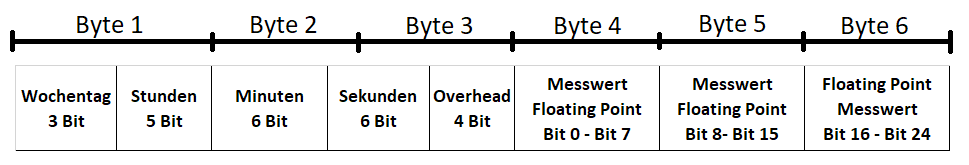
\includegraphics[width=0.9\textwidth]{images/Software_uebertragung.png}
\caption{Übertragungskonzept}
\label{fig:Übertragungskonzept}
\end{center}
\end{figure}

Ein Datenpaket besteht somit aus 6 Byte bzw. 48 Bit. Die Zeitinformationen sind so codiert, dass nur genau so viele Bits zur Verfügung stehen, wie benötigt werden. Im Overhead können zusätzliche Statusinformationen dem Programm übergeben werden bzw. wird dieser benötigt, um ungültige Messdaten zu detektieren (Erklärung später). Ausserdem wird damit der Datenstrom auf ein ganzzahliges Vielfaches von Acht aufgefüllt. Bei den Messdaten spart man sich das letzte Byte der eigentlich 4Byte grossen Fliesskommazahl, da es sich bei diesen Bits um die Grössenordnung 4. - 8. Nachkommastelle handelt. Diese Genauigkeit kann gar nicht erreicht werden, weshalb diese Information auch nicht gespeichert wird.

\subsection{Peripherie und Algorithmen}

Die Funktionen für die Kommunikation mit der Peripherie sowie einige kleine Algorithmen sind zwecks Programmübersicht in externe C-Module gepackt. Auf die Verwendung von externen Bibliotheken ist komplett verzichtet worden. Einerseits um die Nachvollziehbarkeit zu gewährleisten, andererseits, um den Code möglichst optimiert zu gestalten, da dies einer der Hauptprioritäten bei der Erstellung der Firmware war. Es war also nicht Ziel, eine möglichst universell einsetzbare Bibliothek zu schreiben, sondern einen schlanken und effizienten Treiber zu erstellen, der nur gerade die Funktionen beinhaltet, welche das Messgerät benötigt.
 
Der Prozessor muss mit drei Peripheriegeräten kommunizieren. Das erste Modul ist eine RTC, welche am I2C-Bus betrieben wird. Zur Speicherung steht ein Flashspeicher mit SPI Schnittstelle zur Verfügung. Zuletzt das Bluetooth-Modul, über das eine serielle Schnittstelle (USART) emuliert wird. Alle drei Schnittstellen hat der ATMega2560 bereits eingebaut. Sie können mit relativ geringem Aufwand genutzt werden. Die Nutzung dieser Schnittstellen auf \glqq Registerebene\grqq{} wird in diesem Bericht nicht erläutert, dafür wird auf das Datenblatt des Prozessors bzw. den Peripheriegeräten verwiesen, welches im Anhang zu finden ist. 

Das letzte C-Modul beinhaltet die Funktionen zur Auswertung der analogen Eingänge sowie die softwaremässige Erkennung der Strombereiche. Der AD-Wandler ist beim Prozessor bereits integriert und gehört nicht zur Peripherie. Trotzdem sind zwecks Codeübersicht diese Funktionen ausgelagert. Die Funktionsweise aller Module wird im Folgenden erläutert.

\subsubsection*{Bluetooth-Kommunikation via USART}
Die Kommunikation der Firmware mit der PC Software besteht aus zwei Teilen. Erstens vom PC zum Bluetooth-Modul und zweitens vom Modul zum Prozessor. Der PC und das Modul emulieren eine serielle Schnittstelle. Diese Kommunikation ist unabhängig von der zweiten Stufe und erlaubt sogar Verzögerungen, da das Bluetooth-Modul über einen kleinen Datenbuffer verfügt. Die Konfiguration der beiden Übertragungsstufen (Datenrate, Wortbreite, usw.) ist ebenfalls unabhängig und muss nicht übereinstimmen.  

Die Datenrate bzw. Baudrate muss von beiden Partnern mit einer Genauigkeit von ca. 2\% übereinstimmen, damit die Kommunikation funktioniert. Dies gilt für beide Stufen. Da die USART-Schnittstelle nicht mit einem externen Taktgeber betrieben wird, muss die Baudrate für die Kommunikation von Prozessor zu Bluetooth Modul ein ganzzahliger Teiler der CPU-Clock (16 MHz) sein. Die höchstmögliche Übertragungsrate, welche die Bedingung erfüllt und von beiden Geräten unterstützt wird, ist 38400. Die Wortbreite wird auf dem Standardwert von acht Bit belassen, da sowohl die CPU als auch der Speicher mit dieser Wortbreite arbeiten.
Wie die Daten übertragen werden, ist in Kapitel \ref{subsec:Übertragungskonzept} beschrieben. Die Java-Applikation muss diesen Datenstrom auseinander zu trennen und die Werte korrekt abbilden.  

\subsubsection*{I2C Realtime Clock}
Das verwendete RTC-Modul DS3231 ist ein IC mit integriertem Quarz und I2C-Schnittstelle. Es kann direkt an diesem Datenbus angeschlossen werden. Das dazugehörige C-Modul stellt alle Funktionen zur Verfügung, um die Uhrzeit auszulesen und bei Bedarf eine neue Uhrzeit einzustellen. Das RTC-Modul arbeitet mit BCD-Codierung, weshalb beim Lesen und Speichern der Uhrzeit diese stets in Dezimalwerte gewandelt werden muss.

\subsubsection*{4-Channel-ADC}
Der Mikrocontroller verfügt über diverse analoge Eingänge, welche über einen Multiplexer umgeschaltet und anschliessend quantisiert werden. Insgesamt vier solcher Eingänge werden für das Messgerät benötigt. Welchem Eingang welche Bedeutung zukommt, ist in Abbildung \ref{tab:theoretische_Genauigkeit_der_Messbereiche} zu sehen. Da das Wandeln ein vergleichsweise langsamer Prozess ist, werden bei einer Messung immer nur zwei Eingänge gewandelt: einer für die Spannung und einer der Strombereiche. Die Messbereiche werden softwaremässig ausgewertet und umgeschaltet. Ob sich ein Eingang im Grenzbereich befindet (Overflow bzw. Underflow), wird von einem Algorithmus detektiert. Dieser reagiert bei Bedarf und schaltet den Multiplexer auf einen anderen Messbereich um. Der Algorithmus wird anhand eines Beispiels erläutert.

An den Mess-Shunts sind drei Verstärkerschaltungen für die Strommessung angebracht. Diese sind so konzipiert, dass sie ein Sinussignal im Wertebereich \^{I} bis -\^{I} in den Bereich 0V bis 5V abbilden. Daraus folgt, dass je nach Eingangssignal am Ausgang der Verstärkerstufe ein übersteuertes oder ein zu schwaches Signal auftritt. Da das Signal einen Offset aufweist, bedeutet ein Eingangssignal von 2.5V, dass im Moment kein Strom fliesst. In Abbildung \ref{fig:Software_messbereich} ist dieses Verhalten visualisiert.

\begin{figure}[H]
\begin{center}
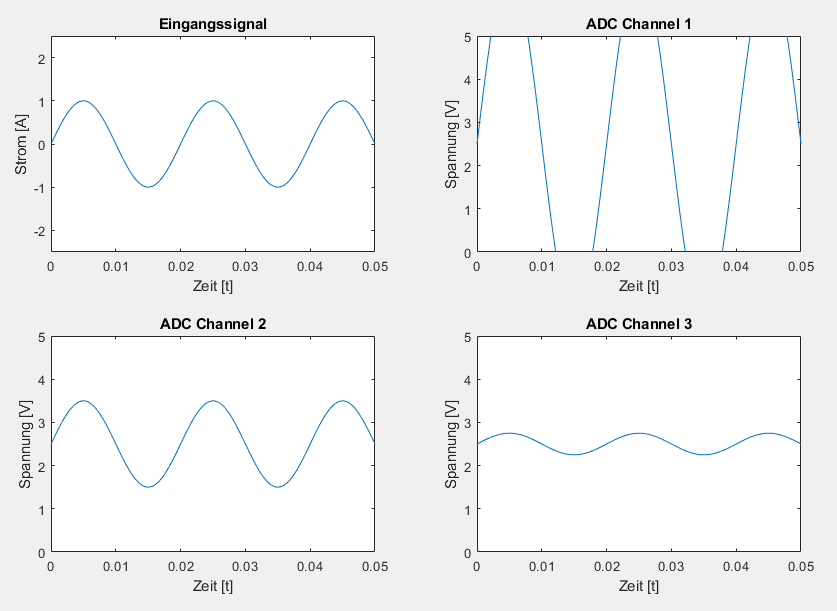
\includegraphics[width=0.9\textwidth]{images/Software_messbereich.png}
\caption{Messbereiche}
\label{fig:Software_messbereich}
\end{center}
\end{figure}

Gegeben ist ein Eingangssignal mit einer Amplitude von 1A. ADC1. Der Eingang für den kleinsten Bereich, übersteuert in diesem Fall und ADC3 schwankt nur gerade so um den Mittelwert des AD-Bereiches. Für die Software bedeutet dies, dass im Falle eines Overflows der ADC immer wieder den Wert 0 oder 1023 zurückliefert. Im Falle des Underflows erhält das Hauptprogramm Werte im Bereich von 512. Dieses Verhalten kann detektiert und ausgewertet werden. Der Algorithmus zählt die Anzahl an \glqq Overflow-Durchgängen \grqq{} bzw. die Anzahl der  \glqq Underflow-Durchgänge\grqq{} . Ist das Signal ausserhalb dieser Bereiche, werden die gezählten Durchgänge wieder dekrementiert. Überschreitet der Zähler einen definierten Wert, wird der Multiplexer umgeschaltet und somit ein anderer analoger Eingang ausgewertet. Die Anzahl an Durchgänge ist Erfahrungssache und wurde experimentell bestimmt. 

[Hier Zahlen]

Hinweis: Der Nullwert von 512 ist nur theoretisch. Welcher Wert die verschiedenen Messbereiche liefern, wird ebenfalls experimentell bestimmt und in der Software entsprechend korrigiert.

\subsubsection*{SPI Flashspeicher}

Dieses C-Modul hat die Aufgabe, den Speicher des Messgerätes zu jeder Zeit konsistent zu halten. Beim Speichern von neuen Messwerten muss die Speicheradresse immer wieder inkrementiert werden. Im Falle, dass der Speicher voll ist, müssen neue Sektoren wieder gelöscht und bereitgestellt werden. Beim Aufstarten muss der Code den zuletzt verwendeten Speicherplatz wiederfinden, unabhängig davon, zu welchem Zeitpunkt das Messgerät vom Strom getrennt wurde. Um all dies sicherzustellen, sind diverse Mechanismen entwickelt und implementiert. Die grösste Aufmerksamkeit gebührte der Effizienz des Codes. 

Der erste Schritt wird mit der Organisation des Speichers getätigt. Der insgesamt 221 Bit (2 MBit) grosse Speicher wird in 64 4KByte-Sektoren unterteilt. Dies ist zugleich die kleinste Einheit, welche gelöscht werden kann (Flashspeicher können nicht byteweise gelöscht werden). Der gesamte Speicher kann mit einer 24Bit-Adresse adressiert werden, wobei effektiv nur 18 Bit benötigt werden. Eine Adresse adressiert jeweils 8 Bit des Speichers. Die Aufteilung ist in Abbildung \ref{fig:Aufteilung_des_Speichers} zu sehen. 

\begin{figure}[H]
\begin{center}
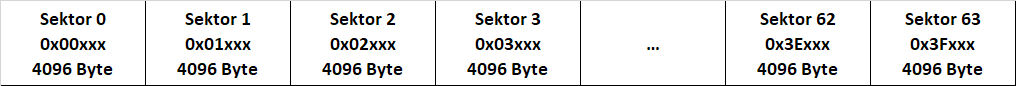
\includegraphics[width=0.9\textwidth]{images/Software_Tabelle_2.png}
\caption{Aufteilung des Speichers}
\label{fig:Aufteilung_des_Speichers}
\end{center}
\end{figure}

Jeder Sektor wird gleich beschrieben: Jeweils die ersten und letzten zwei Bytes sind reserviert und werden nicht mit Messdaten belegt. Das erste Byte eines jeden Sektors wird genutzt, um Statusinformationen über den Sektor zu speichern. Ab Byte Nr. 2 (Indexierung bei 0) beginnen dann die Messdaten, welche nach dem definierten Protokoll jeweils 6 Byte gross sind. Der Sektor endet somit bei Byte Nr. 4093, gefolgt von zwei leeren Speicherplätzen. Insgesamt können somit 682 Messungen pro Sektor abgelegt werden. Sind alle Sektoren voll, wird der erste Sektor gelöscht und darauf weitergeschrieben. In Abbildung \ref{fig:Aufteilung_eines_Sektors} ist die Aufteilung eines einzelnen Sektors zu sehen.

\begin{figure}[H]
\begin{center}
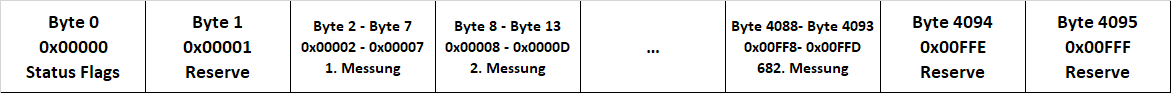
\includegraphics[width=0.9\textwidth]{images/Software_Tabelle_3.png}
\caption{Aufteilung eines Sektors}
\label{fig:Aufteilung_eines_Sektors}
\end{center}
\end{figure}

Der Gewinn dieser Organisation liegt in der Beschleunigung des Initialisierungsvorgangs. Um den zuletzt genutzten Sektor zu finden, ist es ausreichend, jeweils das erste Byte eines Sektors einzulesen. Um den aktuellen Speicherplatz zu finden, muss nur ein Byte pro Messung gelesen werden, nämlich das Byte mit der Overheadinformation. Somit muss bei der Suche des Speicherplatzes nur jedes 6. Byte gelesen werden. Im \glqq worst case\grqq{}  ist der Initialisierungsvorgang also nach 746 Lesevorgängen beendet (64 Statusbytes und 682 Overheads).

Die 4Bit des Overheads wurden so definiert, dass eine Einserfolge einen ungültigen Datensatz signalisiert. Ein leerer Speicherplatz im Flashspeicher ist logisch mit Einsen gefüllt. Das Lesen eines leeren Speicherplatzes gibt den Wert \glqq 1111 1111\grqq{}   zurück. Stösst der Algorithmus beim Aufstarten auf eine Einserfolge im Overhead, ist der leere Speicherplatz gefunden. 

Die Handhabung der Statusinformation eines Sektors ist etwas komplexer und wird im Folgenden genauer erläutert. Der Status wird immer in das gleiche Byte geschrieben. Ein Überschreiben im eigentlichen Sinne ist grundsätzlich nicht möglich. Wie oben erwähnt ist ein leerer Speicherplatz mit logischen Einsen gefüllt. Solange die einzelnen Bits von logisch 1 auf logisch 0 wechseln, ist ein Überschreiben möglich. Sind die Statusinformationen so gewählt, dass sie in der chronologischen Reihenfolge ihres Auftretens nur weitere Nullen hinzufügen, so können mehrere Statusinformationen im gleichen Byte gespeichert werden. Um den Speicher konsistent zu halten, werden nur vier unterschiedliche Zustände benötigt.

\begin{table}[H]
\begin{center}
\begin{tabular}{|l|l|}
\hline
Bitfolge des Statusbytes & Bedeutung \\ \hline
11111110                 & Empty     \\ \hline
11111100                 & Written   \\ \hline
11111000                 & Full      \\ \hline
11110000                 & Busy      \\ \hline
\end{tabular}
\caption{Codierung des Overheades}
\label{tab:Codierung_des_Overheades}
\end{center}
\end{table}

Um Fehlauswertungen zu vermeiden, wird einer Bitfolge aus lauter Einsen oder Nullen keine Bedeutung zugewiesen. 

Anmerkung: Wird unmittelbar nach dem Starten eines Löschvorgangs das Messgerät vom Strom getrennt, wäre es theoretisch möglich, dass beim Lesen des Statusbytes eine Einserfolge (leerer Speicherplatz) zurückgegeben wird. Weiss man aber über das Auftreten dieses Ereignisses bescheid, kann der Initialisierungsvorgang dementsprechend programmiert werden.

\begin{table}[H]
\begin{tabular}{ll}
Empty:			&   Der Sektor ist gelöscht und bereit, um neue Daten 								aufzunehmen. Dieser \\
				&   Status wird nur bei einer 														kompletten Löschung des gesamten Speichers auf alle \\
				&	Sektoren geschrieben.\\
Written:		&   Der Sektor ist mit Daten gefüllt jedoch noch nicht 						voll. Beim Vorbereiten eines \\
				&   neuen Sektors wird 	jeweils direkt der Written-Status 							auf den Sektor geschrieben,\\
				&   auch wenn sich noch keine eigentlichen 										Messdaten darauf befinden.\\
Full:			&   Der Sektor ist komplett mit Messdaten gefüllt.\\
Busy:			&   Der Sektor steht gerade kurz vor einem Löschvorgang.\\
\end{tabular}
\end{table}

Der Busy-Status ist deswegen notwendig, weil ein Löschvorgang vergleichsweise langsam ist (bis zu 50 ms). Erst nach dem Abschliessen des Löschvorgangs wird dem Sektor ein neuer Status zugewiesen.

Um beim Aufstarten nun den korrekten Sektor zu finden, bedarf es der korrekten Interpretation der Statusinformationen. Was wenn während des Schreibvorgangs der Strom getrennt wird? Was wenn genau beim \glqq wrap around\grqq{}   das Gerät ausgeschaltet wird? Es gibt eine grosse Zahl von Ereignissen, welche auftreten können. Viele davon sind Spezialfälle, welche nur sehr selten sind. Trotzdem müssen diese abgedeckt sein. Hier ein einfaches Beispiel:

Das Messgerät war kurze Zeit im Betrieb gewesen. Die ersten drei Sektoren sind bereits voll. Genau als der dritte Sektor voll ist, ist das Messgerät ausgesteckt worden. Der vierte Sektor und alle darauffolgenden Sektoren haben somit als Status \glqq Empty\grqq . Die ersten drei Sektoren den Status  \glqq Full\grqq .

Beim Aufstarten wird daher prioritär zuerst nach leeren Sektoren gesucht. Danach nach beschriebenen Sektoren und entgegen der Reihenfolge von Abbildung \ref{tab:Codierung_des_Overheades} werden Sektoren mit dem Status \glqq Busy\grqq{}  noch vor Sektoren mit dem Status \glqq Full\grqq{}  gesucht.

Im genannten Beispiel findet der Algorithmus schnell einen Treffer und liefert als Ergebnis den Dezimalwert 3 für den vierten Sektor (Indexierung startet bei 0!). Nun muss der Algorithmus das Statusbyte des vorherigen Sektors überprüfen. Er wird als Ergebnis den Status \glqq Full\grqq{} bekommen. Nun ist die Information eindeutig und das Programm weiss, dass der Sektor mit der Nummer 3 der aktuelle Sektor zum Schreiben ist. Da dieser leer ist, kann die Suche nach dem Speicherplatz gestoppt werden und als Nummer für den aktuellen Speicherplatz der Wert 2 gesetzt werden. (2 deshalb, weil immer beim dritten Byte begonnen, wird Messdaten zu schreiben)

Dies ist nur ein Beispiel. Der gesamte Initialisierungsablauf ist in Abbildung \ref{tab:Rückgabewert} zu sehen. Die rot eingefärbte Linie ist der Hauptpfad und signalisiert den Normalablauf des Speicherns. Der Algorithmus liefert einen 8Bit-Wert zurück. Die ersten 6 Bit repräsentieren den Index des gefundenen Sektors, die obersten beiden Bits werden für die Codierung der Statusinformation verwendet, damit das Hauptprogramm weiss, welche Art von Status zuerst gefunden wurde. Die Codierung ist in der nachfolgenden Tabelle zu sehen.


\begin{table}[H]
\begin{center}
\begin{tabular}{|l|l|}
\hline
Rückgabewert des Algorithmus & Bedeutung                                                                                                                                                                            \\ \hline
00xxxxxx                     & Es wurden noch leere Sektoren gefunden.                                                                                                                                              \\ \hline
01xxxxxx                     & \begin{tabular}[c]{@{}l@{}}Es gibt keine leeren Sektoren mehr, aber\\ es wurde ein beschriebener Sektor gefunden.\\ (Normalzustand)\end{tabular}                                     \\ \hline
10xxxxxx                     & \begin{tabular}[c]{@{}l@{}}Es wurden weder leere noch beschriebene Sektoren\\ gefunden. Aber es wurde ein Sektor gefunden,\\ welcher noch nicht korrekt gelöscht wurde.\end{tabular} \\ \hline
11111111                     & Alle Sektoren sind voll.                                                                                                                                                             \\ \hline
\end{tabular}
\caption{Rückgabewert des Algorithmus}
\label{tab:Rückgabewert}
\end{center}
\end{table}

[ Grafik folgt noch ] 

Zuletzt nochmals eine schnelle Zusammenfassung:

Das Programm muss sich zur Laufzeit nur zwei Variablen merken. Den aktuellen Sektor und die aktuelle Nummer des Speicherplatzes. Daraus kann jeweils die korrekte 24Bit-Adresse gebildet werden. Beim Aufstarten sucht sich ein Algorithmus diese beiden Werte und gibt sie ans Hauptprogramm weiter. Durch die Speicherorganisation ist dieser Suchvorgang sehr effizient und benötigt nur wenige Lesevorgänge. Die Speicherplatznummer wird stetig inkrementiert. Ist ein Sektor voll, so wird die Sektornummer inkrementiert und die Nummer des Speicherplatzes wieder auf 2 gesetzt. Ist der gesamte Speicher voll, so wird nach und nach der nächste Sektor wieder gelöscht, um darauf neue Daten zu schreiben. Im Dauerbetrieb gehen dadurch die ältesten Messdaten stetig verloren. 


\pagebreak
\subsection{Bediensoftware}%Elias 1 Seite
%Topdown beschreibung
Als Bediensoftware ist ein Java-Applikation geschrieben worden. Diese soll den Benutzern die Möglichkeit bieten, die gemessenen Daten auszulesen und in ein gebräuchliches Format zu exportieren, damit eine einfache Weiterverarbeitung der Daten ermöglicht beispielsweise in Excel oder Matlab.

Das Programm bietet drei Hauptfunktionen um mit dem P3T7 zu kommunizieren. Diese sind im Bereich 'Steuerung' zu finden. Daneben bietet das Tool die Funktion sich mit dem P3T7 zu verbinden. Die im Bereich 'Bluetooth' zu finden ist. Die restlichen Elemente dienen alle der Ausgabe. Der 'Status' visualisiert den Fortschritt des Downloads. Im Bereich 'Echtzeit' werden die aktuellen Messwerte des P3T7 angezeigt. Im dominierenden Bereich 'Plot' werden die Daten aus dem Speicher visualisiert, um dem Benutzer eine schnelle Validierung der Daten zu ermöglichen.

\begin{figure}[H]
\begin{center}
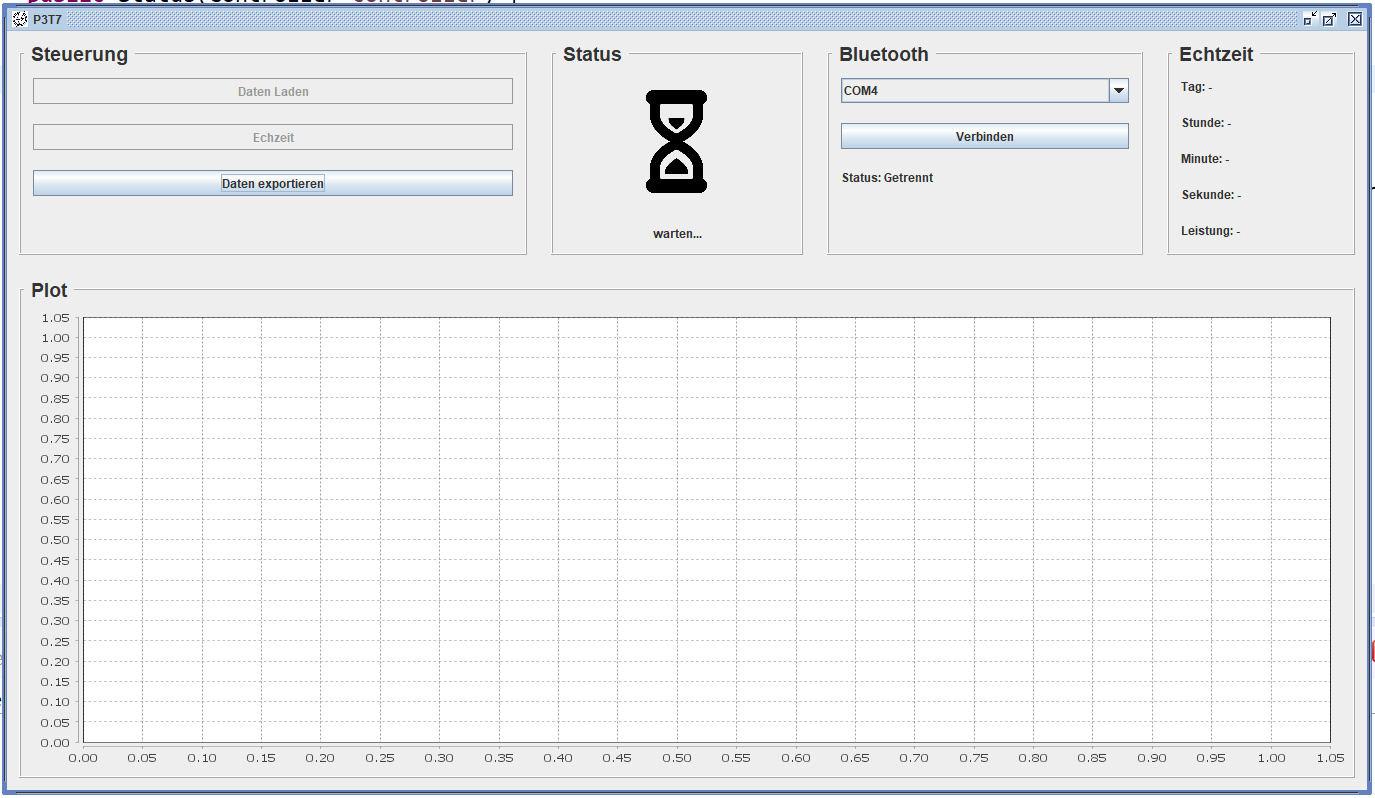
\includegraphics[width=0.9\textwidth]{images/Software_GUI.png}
\caption{GUI der Bediensoftware}
\end{center}
\end{figure}

\subsubsection*{Steuerung}

Mit den drei Hauptfunktionen können die Daten aus dem P3T7 extrahiert werden. Wenn ein Download gestartet wird, kann auf dem Status-Panel der Fortschritt beobachtet werden. Falls der Download abgeschlossen ist werden die Daten im Plot dargestellt. Dieser soll dem Nutzer die Sicherheit geben, dass keine falschen Daten heruntergeladen wurden. Anschliessend kann mit dem Button 'Daten exportiern' ein CSV-File generiert werden. Dieses ist mit dem Namen 'ausgabe.txt' neben der Programmdatei zu finden. Mit dem Button 'Echtzeit' kann die Echtzeitübertragung gestartet werden. Während der Echtzeitübertragung werden jede Sekunde die aktuellen Messwerte an das Tool weitergeleitet. Diese werden anschliessend direkt im Echtzeit-Panel angezeigt.

\subsubsection*{Bluetooth}

Das Bluetoot-Modul emuliert über Bluetooth eine seriell Verbindung. Um das Tool mit dem P3T7 zu verbinden muss zuerst im Betriebssystem das P3T7 gekoppelt werden.  Ist dies erfolgt kann im Tool im Bluetooth-Panel aus dem Dropdown-Menü der entsprechende ComPort ausgewählt werden. Dieser kann im Gerätemanager nachgeschaut werden. Falls ein falscher Port ausgewählt wird, vergeht eine Zeit (ca. 30s) bis das Programm den Fehler bemerkt, welche abgewartet wird.


\subsubsection*{Programmstruktur}

Das Programm wurde nach dem MVC Pattern realisiert. Somit hat es praktisch keine nennenswerten strukturellen Eigenheiten bis auf das Interface für die serielle Verbindung. 

\begin{figure}[H]
\begin{center}
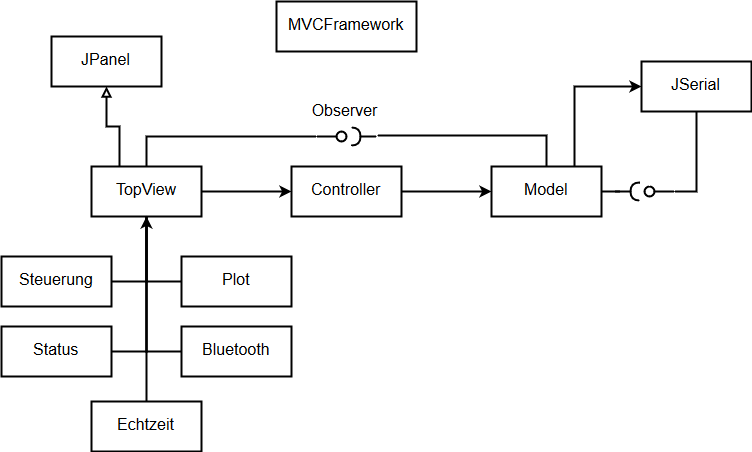
\includegraphics[width=0.9\textwidth]{images/Software_UML.png}
\caption{Diagramm der Bediensoftware}
\end{center}
\end{figure}

\input{input/Qualitätssicherung}
\section{Schlusswort}%Beni 1 Seite
\section{Anhang}
\cite{Mason1953,Mason1956}

\subsection*{Bibliographie}
\bibliographystyle{fhnwreport/IEEEtran}

\bibliography{input/bibliographie,fhnwreport/IEEEabrv}
%%%%%%%%%%%%%%%%%%%%%%%%%%%%%%%%%%%%%%%%%%%%%%%%%%%%%%%%


\end{document}

